\documentclass[pdflatex,sn-basic,Numbered,iicol]{sn-jnl}

% Springer Nature LaTeX template configured for Computational Mechanics (Journal ID 466):
% - [iicol] selects the two-column layout required by Computational Mechanics
% - [sn-basic,Numbered] formats square-bracket numbered citations [1], [1-3, 7] with full DOI URLs
% Note: sn-jnl.cls preloads hyperref, appendix, amsthm, natbib, rotating, and threeparttable.
\usepackage{graphicx}
\usepackage{multirow}
\usepackage{amsmath,amssymb,amsfonts}
\usepackage{mathrsfs}
\usepackage{xcolor}
\usepackage{textcomp}
\usepackage{manyfoot}
\usepackage{booktabs}
\usepackage{bm}
\usepackage{mathtools}
\usepackage{enumitem}

% sn-jnl.cls loads article with [fleqn]; zeroing \mathindent gives equations
% the full 76 mm column width in [iicol] mode so tags never collide.
\setlength{\mathindent}{0pt}
\hypersetup{hypertexnames=false}

% Barred and bold notation macros
\newcommand{\bmx}{\bm{x}}
\newcommand{\bmk}{\bm{k}}
\newcommand{\bmu}{\bm{u}}
\newcommand{\bmv}{\bm{v}}
\newcommand{\bmK}{\bm{K}}
\newcommand{\bmM}{\bm{M}}
\newcommand{\bmB}{\bm{B}}
\newcommand{\bmR}{\bm{R}}
\newcommand{\bmT}{\bm{T}}
\newcommand{\bmC}{\bm{C}}
\newcommand{\barw}{\bar{\omega}}
\newcommand{\bark}{\bar{k}}
\newcommand{\ellbar}{\bar{\ell}_{\mathrm{i}}}
\newcommand{\dif}{\mathrm{d}}
\newcommand{\iu}{\mathrm{i}}

\raggedbottom

\begin{document}

\title[Orientation-Dependent Dispersion and Wave Steering in 2D Strain-Gradient Elasticity]{Orientation-Dependent Dispersion and Wave Steering in Two-Dimensional Strain-Gradient Elasticity: Directional Spectral Separation versus Complete Bragg Gaps under Material Contrast}

% Corresponding author ORCID: 0000-0002-5238-1963 (https://orcid.org/0000-0002-5238-1963)
\author*[1]{\fnm{Vipin} \sur{Gupta}}\email{vipin@gurugramuniversity.ac.in}

\affil*[1]{\orgdiv{Department of Mathematics}, \orgname{Gurugram University}, \orgaddress{\city{Gurugram}, \postcode{122505}, \state{Haryana}, \country{India}}}

\abstract{This paper investigates direction-dependent wave dispersion in two-dimensional strain-gradient elasticity when the wavelength approaches an intrinsic material length scale. The formulation combines a rotated ellipsoidal characteristic-length tensor, defined by the orientation $\theta$ and aspect ratio $\mathrm{AR}$, with local Mindlin Form-II elasticity and independent gradient micro-inertia. The Bloch--Floquet problem is discretized using a conforming 32-degree-of-freedom Bogner--Fox--Schmit element, with the Bloch phase applied consistently to displacement and derivative degrees of freedom. In the homogeneous case, orientation and aspect ratio modify the dispersion branches and produce a directional spectral separation along $\Gamma$--$X$. Its maximum value is 0.0677 at zero orientation and $\mathrm{AR}=7$. The complete-gap measure remains negative for all sampled configurations, with maximum orientation sensitivity at $\mathrm{AR}=10$. This separation is a reduced-zone property of the homogeneous medium and does not represent Bragg attenuation. On the acoustic branch, rotation of the characteristic-length tensor deflects the group velocity from the wave vector by up to $2.78^\circ$. The peak deviation remains invariant to within $10^{-5}$ degrees over the sampled orientations. In contrast, the heterogeneous epoxy--YBCO cell exhibits a positive complete Bragg gap of 43.94\% on the coarsest mesh. The gap narrows systematically with refinement and remains mesh-unconverged. Gradient micro-inertia bounds the high-wavenumber phase speed of the branch considered. The results show that orientation controls the direction of energy transport in a homogeneous strain-gradient medium, whereas complete attenuation requires material contrast.}

\keywords{Strain-gradient elasticity, Bogner--Fox--Schmit finite element, Bloch--Floquet dispersion, Gradient micro-inertia, Wave steering, Phononic Bragg band gaps}

\maketitle

\section{Introduction}
\label{sec:intro}

Periodic elastic media can be designed to control wave propagation through their dispersion. Early calculations established band structures for periodic composites; experiments and theory later showed that two-dimensional solids can support absolute acoustic gaps \cite{SigalasEconomou1992,kushwaha1993,vasseur2001}. Lattice analyses and topology-optimization studies have since used geometry to tailor pass bands, stop bands, and wave transmission \cite{MartinssonMovchan2003,SigmundJensen2003,Dalklint2022}. Recent methods target gaps at specified frequencies and use multiple materials to control gap formation, while scaling studies track how optimized gaps shift with structural size \cite{He2026,Nakayama2025,Quinteros2026}. Reviews cover phononic-crystal mechanisms, engineered band gaps, and applications \cite{Vasileiadis2021,Oudich2023,MaWangYuan2026}. A gap along selected directions does not guarantee a complete gap; the latter requires suppression throughout the Brillouin zone.

When a wavelength approaches the material's microstructural scale, a local Cauchy law may not capture size-dependent stiffness or dispersion. Higher-order theories add kinematic measures and their work-conjugate stresses. Their development draws on couple-stress and microstructure theories, second-gradient elasticity, and variational treatments of higher-order boundary work \cite{toupin1962,MindlinTiersten1962,mindlin1964,Mindlin1965,mindlineshel1968,Germain1973}. Later studies examined strain-gradient descriptions of nonuniform deformation and small-scale beam experiments \cite{Aifantis1999,YangChongLamTong2002,LamYangChongWangTong2003}. Reviews and lattice-based derivations describe other formulations of gradient elasticity \cite{askesaifantis2011,polyzosfotiadis2012}. We use the local Mindlin Form-II theory; nonlocal integral and micromorphic theories are related approaches, but they are distinct formulations.

A dynamic gradient model needs a kinetic-energy law as well as gradient stiffness. With classical inertia alone, the shear branch examined here has phase speed proportional to wavenumber at high wavenumbers. Independent gradient micro-inertia gives this branch a finite high-wavenumber limit. That result follows from the constitutive and kinetic-energy laws used here; other higher-order continua need not have the same limit. One-dimensional studies have examined dispersion in gradient-elastic beams and periodic media, including dipolar-gradient formulations \cite{papargyribeskou2009,liweizhou2016,HosseiniSladekSladekZhang2024}. A two-dimensional phononic crystal has also been analyzed with a relaxed micromorphic model that includes free and gradient micro-inertia \cite{MadeoColletMiniaciBillonOuisseNeff2018}. Together, these studies show that the continuum and inertia laws affect the interpretation of short-wavelength bands, although their constitutive models differ from the local Mindlin Form-II model used here.

Size-dependent phononic-crystal studies use a range of constitutive models. Transfer-matrix analyses show that imperfect interfaces can alter one-dimensional band gaps \cite{zhengwei2009}. Other one-dimensional work considers dipolar-gradient elasticity, gradient thermoelasticity, and flexoelectric strain-gradient coupling \cite{liweizhou2016,li2023anchorA,li2024anchorB,HosseiniSladekSladekZhang2024}. In two dimensions, researchers have applied nonlocal strain-gradient theory to nanoscale phononic crystals and studied mixed and defect modes in a phononic-crystal slab \cite{JinHuHu2022,JinHuHu2023}. Other model-specific comparisons include thermoelastic cylindrical crystals and functionally graded lattices \cite{hosseinizhang2021,mishra2026anchorC}. Anisotropy and orientation have also been studied in conventional phononic crystals: work on orthotropic fillers and anisotropic plates reports shifts in band locations and widths as material axes or inclusions rotate relative to the lattice \cite{zhanwei2010,YaoWuHouXin2011}. Recent studies examine direction-dependent gaps in anisotropic nanocrystal assemblies and the effects of anisotropic constituents in optimized phononic crystals \cite{Kim2023,Liu2024anisotropic}. For flexural plate waves, anisotropic equal-frequency contours can align group velocity with a lens interface over a broad frequency range \cite{Danawe2023}. Prior work has therefore established orientation-dependent band tuning. Here I examine how an oriented characteristic-length tensor affects dispersion and energy-flow direction in a local two-dimensional strain-gradient model with gradient micro-inertia.

The finite-element approximation must also accommodate the strain-gradient weak form. Because it contains second derivatives of displacement, the trial space must be $H^2$-conforming or use an equivalent mixed formulation. The bicubic Bogner--Fox--Schmit (BFS) rectangle provides $C^1$ continuity across elements on structured quadrilateral meshes \cite{bfs1965}. Earlier studies developed displacement-based, mixed, and implicit-gradient finite elements \cite{ShuKingFleck1999,AmanatidouAravas2002,ZervosPapanicolopulosVardoulakis2009,Beheshti2017}. Later work treats second-gradient boundary-value problems, higher-order Hermite mappings on regular and distorted domains, mixed elements with patch recovery or shared degrees of freedom, and mixed crack formulations \cite{AndreausDellIsolaGiorgioPlacidiLekszyckiRizzi2016,BacciocchiFantuzzi2023,BacciocchiFantuzzi2025,ChoiLeeSim2023,Papanicolopulos2024,ChirkovNazarenkoAltenbach2024}. For a conforming BFS Bloch element, the same phase transformation must be applied to displacement values and all derivative degrees of freedom, including the mixed derivative.

To my knowledge, the cited literature does not report a two-dimensional Bloch--Floquet finite-element framework that combines a rotated ellipsoidal characteristic-length tensor, local Mindlin Form-II strain-gradient elasticity with independent gradient micro-inertia, and a conforming $C^1$ BFS discretization with phase transformations on all relevant degrees of freedom. This study addresses that combination and builds on established work on anisotropy, orientation effects, and size-dependent phononic crystals. It makes four contributions:
\begin{itemize}
  \item We formulate a Bloch--Floquet framework for two-dimensional anisotropic strain-gradient elasticity. The rotated ellipsoidal averaging domain defines the length tensor, with aspect ratio $\mathrm{AR}=l_1/l_2$ and orientation $\theta$ as separate design variables.
  \item Gradient micro-inertia is examined analytically and numerically. For the branch studied, $\ell_{\mathrm{i}}=0$ gives an unbounded high-wavenumber phase speed, whereas $\ell_{\mathrm{i}}>0$ yields the finite limit $v_{T,\infty}=\sqrt{\mu/\rho}\,l_{\mathrm{eff}}/(\sqrt{10}\,\ell_{\mathrm{i}})$ derived in Appendix~\ref{app:asymptotics}.
  \item A conforming 32-degree-of-freedom BFS element is developed, with the same complex Bloch phase applied to displacement, first derivatives, and the mixed derivative.
  \item Across the $(\theta,\mathrm{AR})$ design space, I evaluate directional dispersion, gap measures, and group velocity. The energy-flux relation follows from local balance; the analysis also separates directional spectral separations from complete gaps and measures steering amplitude and lobe orientation.
\end{itemize}

{\sloppy
The homogeneous case treated here is analyzed on an artificial Bloch periodic cell with no physical material contrast. The resulting path-specific spectral separation is therefore a reduced-zone effect of the underlying continuum, not a Bragg-type attenuation gap; this empty-lattice construction and its distinction from a genuine Bragg gap in anisotropic media has been analyzed by Wang, Maznev, and Laude \cite{WangMaznevLaude2016}. Frequency-dependent directional beam steering has separately been studied for periodic lattices using homogenized continuum descriptions, for instance in the hexagonal-lattice continuum model of Rosi and Auffray \cite{RosiAuffray2019}. The present contribution is the joint treatment. One homogeneous model quantifies orientation-dependent reduced-zone spectral separation and group-velocity steering, and the corresponding materially-contrasted case is shown separately to support a genuine complete Bragg gap, so the two mechanisms remain distinct.
\par}


\section{Anisotropic Strain-Gradient Continuum with Micro-Inertia}
\label{sec:continuum}

\subsection{Ellipsoidal characteristic-length tensor}
In standard isotropic gradient elasticity, the microstructural influence is often represented by a scalar length scale $l$. Under plane strain, I describe an oriented microstructure by its in-plane elliptical averaging neighborhood $\mathcal{E}_0$, with principal semi-axes $l_1$ and $l_2$:
\begin{equation}
\mathcal{E}_0 = \left\{ (x_1', x_2') \in \mathbb{R}^2 \;\middle|\; \frac{(x_1')^2}{l_1^2} + \frac{(x_2')^2}{l_2^2} \le 1 \right\},
\label{eq:ellipse_def}
\end{equation}
where $(x_1', x_2')$ are local principal coordinates aligned with the microstructural axes. We define the in-plane characteristic-length tensor as the diagonal matrix of squared semi-axes. This model definition differs from the normalized covariance tensor of a uniformly filled two-dimensional ellipse:
\begin{equation}
\mathbf{L}_0 = \begin{bmatrix} l_1^2 & 0 \\ 0 & l_2^2 \end{bmatrix}.
\label{eq:L0_mat}
\end{equation}

We hold the area $\pi l_1l_2$ fixed as the aspect ratio varies, using an isotropic baseline $l_{\mathrm{iso}}>0$:
\begin{equation}
\begin{split}
l_1 &= l_{\mathrm{iso}}\sqrt{\mathrm{AR}}, \quad l_2 = \frac{l_{\mathrm{iso}}}{\sqrt{\mathrm{AR}}}, \\
\pi l_1l_2 &= \pi l_{\mathrm{iso}}^2, \\
\det(\mathbf{L}_0) &= l_1^2l_2^2 = l_{\mathrm{iso}}^4 = \mathrm{const},
\end{split}
\label{eq:volume_equivalent}
\end{equation}
where $\mathrm{AR} = l_1/l_2 \ge 1$ is the microstructural aspect ratio. The factor $1/10$ is a normalization set by the three-dimensional second moment of the solid-ellipsoid averaging domain; it reduces to the classical scalar-length limit of Mindlin Form-II gradient elasticity when $l_1=l_2$, only the in-plane length components enter the plane-strain tensor, and the same factor is used wherever the characteristic-length tensor enters the formulation (Eqs.~\eqref{eq:double_stress} and~\eqref{eq:Kg_int}, and Appendix~\ref{app:asymptotics}).

\subsubsection{Orientation convention and passive rotation}
We take positive $\theta$ to denote a clockwise orientation of the principal axes relative to the global frame $(x_1,x_2)$. The passive map from global coordinates $\bmx$ to local principal coordinates $\bmx'$ is:
\begin{equation}
\bmx' = \bmR(\theta)\bmx, \quad \bmR(\theta) = \begin{bmatrix} \cos\theta & -\sin\theta \\ \sin\theta & \cos\theta \end{bmatrix}.
\label{eq:R_matrix}
\end{equation}
Under this coordinate transformation, the characteristic-length tensor in the global frame is:
\begin{equation}
\setlength{\arraycolsep}{3pt}
\begin{split}
\mathbf{L}(\theta) &= \bmR(\theta)^\mathsf{T} \mathbf{L}_0 \bmR(\theta) \\
&= \begin{bmatrix} \cos\theta & \sin\theta \\ -\sin\theta & \cos\theta \end{bmatrix} \begin{bmatrix} l_1^2 & 0 \\ 0 & l_2^2 \end{bmatrix} \begin{bmatrix} \cos\theta & -\sin\theta \\ \sin\theta & \cos\theta \end{bmatrix}.
\end{split}
\label{eq:L_rotation}
\end{equation}
Carrying out the matrix multiplication gives:
\begin{subequations}
\label{eq:L_components}
\begin{align}
L_{11}(\theta) &= l_1^2 \cos^2\theta + l_2^2 \sin^2\theta, \label{eq:L11} \\
L_{22}(\theta) &= l_1^2 \sin^2\theta + l_2^2 \cos^2\theta, \label{eq:L22} \\
L_{12}(\theta) &= L_{21}(\theta) = (l_2^2 - l_1^2)\cos\theta\sin\theta. \label{eq:L12}
\end{align}
\end{subequations}
For an elongated microstructure ($l_1 > l_2$), the off-diagonal coupling $L_{12}(\theta)$ is negative for $0 < \theta < 90^\circ$ and reaches its minimum, $(l_2^2-l_1^2)/2$, at $\theta=45^\circ$. Figure~\ref{fig:ellipsoid_tensor} illustrates the area-preserving averaging ellipses for several aspect ratios and plots the length-tensor components $L_{11}$, $L_{22}$, and $L_{12}$ against orientation. Because $\bmR(\theta)$ is orthogonal, the eigenvalues of $\mathbf{L}(\theta)$ are invariant under rotation:
\begin{equation}
\mathrm{spec}(\mathbf{L}(\theta)) \equiv \{l_1^2, l_2^2\} \quad \forall\,\theta \in [0, 2\pi).
\label{eq:eigenvalues_invariant}
\end{equation}
For $l_1,l_2>0$, $\mathbf{L}(\theta)$ is positive definite at every orientation.

\begin{figure*}[htbp]
\centering
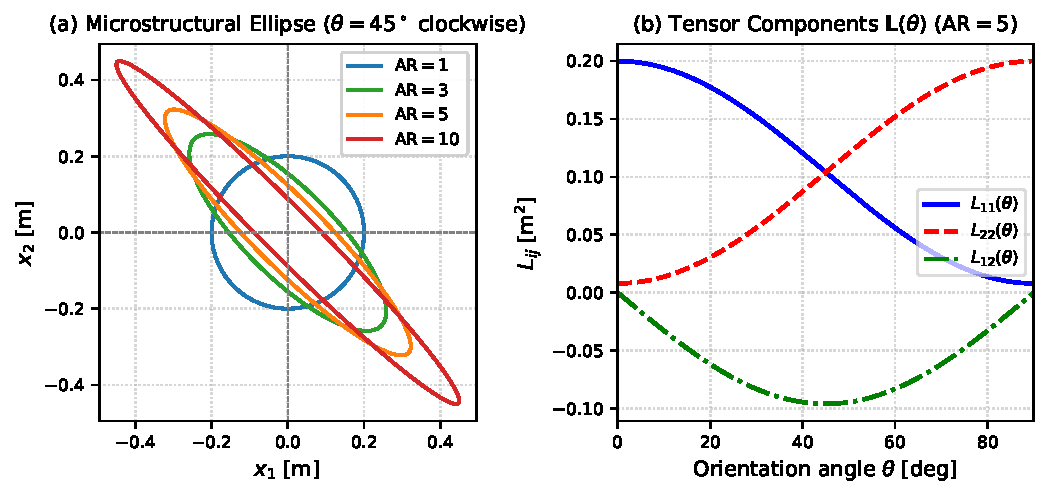
\includegraphics[width=\textwidth]{figures/fig01_ellipsoid_tensor.pdf}
\caption{(a) Area-preserving averaging ellipses at $\theta=45^\circ$ for $\mathrm{AR}=1,3,5,10$, with positive orientation measured clockwise. (b) Length-tensor components versus orientation for $\mathrm{AR}=5$, including $L_{12}(45^\circ)=-0.096\,\mathrm{m}^2$ under the same passive-rotation convention}
\label{fig:ellipsoid_tensor}
\end{figure*}

\subsection{Kinematics and constitutive response}
Assuming infinitesimal deformations under two-dimensional plane-strain conditions ($u_3 = 0, \partial(\cdot)/\partial x_3 = 0$), the classical displacement gradient and infinitesimal strain tensor $\bm\varepsilon$ are:
\begin{equation}
\varepsilon_{ij} = \frac{1}{2}(u_{i,j} + u_{j,i}), \quad i,j \in \{1, 2\}.
\label{eq:strain_def}
\end{equation}
The strain-gradient tensor $\bm\eta$ is the spatial derivative of infinitesimal strain:
\begin{equation}
\eta_{ijk} = \varepsilon_{ij,k} = \frac{1}{2}(u_{i,jk} + u_{j,ik}), \quad \eta_{ijk} = \eta_{jik}.
\label{eq:strain_gradient_def}
\end{equation}
Under plane strain in 2D, $\bm\varepsilon$ has 3 independent components ($\varepsilon_{11}, \varepsilon_{22}, 2\varepsilon_{12}$), and $\bm\eta$ has 6 ($\eta_{111}, \eta_{112}, \eta_{221}, \eta_{222}, 2\eta_{121}, 2\eta_{122}$).

\subsubsection{Mindlin Form-II constitutive law}
In Mindlin's Form II, the strain-energy density $W$ has classical and strain-gradient contributions:
\begin{equation}
W = \frac{1}{2}\sigma_{ij}\varepsilon_{ij} + \frac{1}{2}\tau_{ijk}\eta_{ijk},
\label{eq:strain_energy_W}
\end{equation}
where $\bm\sigma$ is the Cauchy stress tensor and $\bm\tau$ is the third-order double-stress (or dipolar stress) tensor. For an isotropic base material parameterized by Lam\'e constants $\lambda$ and $\mu$, the Cauchy stress satisfies Hooke's law:
\begin{equation}
\sigma_{ij} = C_{ijkl}\varepsilon_{kl} = \lambda \delta_{ij}\varepsilon_{kk} + 2\mu \varepsilon_{ij}.
\label{eq:cauchy_stress}
\end{equation}
The double-stress tensor $\tau_{ijk}$ is conjugate to $\eta_{ijk}$ through the anisotropic gradient-elasticity law involving $\mathbf{L}$:
\begin{equation}
\begin{split}
\tau_{ijk} &= \frac{1}{10} L_{kl} C_{ijmn}\eta_{mnl} \\
&= \frac{1}{10} L_{kl}\left(\lambda \delta_{ij}\eta_{mml} + 2\mu \eta_{ijl}\right),
\end{split}
\label{eq:double_stress}
\end{equation}
For stable isotropic elastic constants ($\mu>0$ and $3\lambda+2\mu>0$) and positive-definite $\mathbf{L}$, the quadratic strain energy is non-negative and vanishes only when both the strain and strain-gradient fields vanish.

\subsubsection{Gradient micro-inertia}
We include gradient micro-inertia in the kinetic-energy density $T$:
\begin{equation}
T = \frac{1}{2}\rho \dot u_i \dot u_i + \frac{1}{2}\rho \ell_{\mathrm{i}}^2 \dot u_{i,j}\dot u_{i,j},
\label{eq:kinetic_energy_T}
\end{equation}
where $\rho$ is the macroscopic mass density and $\ell_{\mathrm{i}} > 0$ is the independent micro-inertia length parameter. Applying Hamilton's principle $\delta \int_{t_1}^{t_2} (T - W)\,\dif t = 0$ yields the strong-form equations of dynamic equilibrium in the bulk:
\begin{equation}
\sigma_{ij,j} - \tau_{ijk,jk} = \rho\left(\ddot u_i - \ell_{\mathrm{i}}^2 \ddot u_{i,jj}\right), \quad \text{in } \Omega.
\label{eq:strong_form}
\end{equation}
The operator $1-\ell_{\mathrm{i}}^2\nabla^2$ increases the effective inertia of spatially varying acceleration. For the shear branch examined here, Section~\ref{sec:microinertia} and Appendix~\ref{app:asymptotics} show that this term bounds the high-wavenumber phase speed.

\subsubsection{Model reductions}
The model has four useful physical limits:
\begin{enumerate}[label=(\roman*)]
  \item \textbf{Classical elasticity limit ($l_{\mathrm{iso}} \to 0$ at fixed finite $\mathrm{AR}$, $\ell_{\mathrm{i}} \to 0$):} Both principal gradient lengths vanish, double stresses vanish, and the classical Navier equations $\sigma_{ij,j}=\rho\ddot u_i$ are recovered with dispersionless acoustic speeds $c_T=\sqrt{\mu/\rho}$ and $c_L=\sqrt{(\lambda+2\mu)/\rho}$.
  \item \textbf{Isotropic gradient elasticity ($\mathrm{AR} = 1$):} Here $l_1 = l_2 = l_{\mathrm{iso}}$, so $L_{11} = L_{22} = l_{\mathrm{iso}}^2$ and $L_{12} = 0$ for all $\theta$, recovering isotropic Form-II gradient elasticity.
  \item \textbf{Gradient elasticity without micro-inertia ($\ell_{\mathrm{i}} = 0$):} Higher-order stiffness remains while dynamic regularization is removed; the transverse branch analyzed in Appendix~\ref{app:asymptotics} then has $v_p\propto k$ as $k\to\infty$.
  \item \textbf{Quarter-turn covariance:} For fixed $l_1,l_2$, a $90^\circ$ change of orientation interchanges the diagonal components and reverses the off-diagonal component: $L_{11}(\theta+90^\circ)=L_{22}(\theta)$, $L_{22}(\theta+90^\circ)=L_{11}(\theta)$, and $L_{12}(\theta+90^\circ)=-L_{12}(\theta)$.
\end{enumerate}

\subsection{Boundary operators}
Let $\Gamma=\partial\Omega$ be a smooth boundary with unit outward normal $\bm n$. For the strain-energy term, integration by parts gives the boundary contribution
\begin{equation}
\begin{split}
\left.\delta\int_\Omega W\,\dif\Omega\right|_\Gamma
={}& \int_\Gamma \Big[(\sigma_{ij}-\tau_{ijk,k})n_j\,\delta u_i \\
&+ \tau_{ijk}n_k\,\delta u_{i,j}\Big] \,\dif\Gamma.
\end{split}
\label{eq:elastic_boundary_work}
\end{equation}
On a smooth boundary, decomposing $\delta u_{i,j}$ into normal and tangential parts and integrating the tangential part by parts gives the work-conjugate double traction and effective elastic traction:
\begin{equation}
\begin{split}
R_i &= n_jn_k\tau_{ijk}, \\
p_i^{\mathrm{el}} &= (\sigma_{ij}-\tau_{ijk,k})n_j - \nabla_j^S(n_k\tau_{ijk}),
\end{split}
\label{eq:traction_def}
\end{equation}
where $\nabla_j^S$ denotes the surface divergence acting on the tangential projection of $n_k\tau_{ijk}$; additional line forces arise at boundary edges. The gradient micro-inertia adds $\rho\ell_{\mathrm{i}}^2\ddot u_{i,j}n_j$ to the dynamic traction, so $p_i^{\mathrm{dyn}}=p_i^{\mathrm{el}}+\rho\ell_{\mathrm{i}}^2\ddot u_{i,j}n_j$. The work-conjugate pairs are $(u_i,p_i^{\mathrm{dyn}})$ and $(\partial u_i/\partial n,R_i)$. On Bloch-paired cell faces, the kinematic phase constraints replace independent free-boundary conditions.

\section{Bloch--Floquet formulation and observables}
\label{sec:bloch}

\subsection{Square lattice and Bloch conditions}
We generate the two-dimensional periodic medium by translating the square cell $\Omega_{\mathrm{cell}}=[0,L]\times[0,L]$ along
\begin{equation}
\bm{a}_1=\begin{bmatrix}L\\0\end{bmatrix},\qquad
\bm{a}_2=\begin{bmatrix}0\\L\end{bmatrix}.
\label{eq:lattice_vectors}
\end{equation}
The corresponding reciprocal vectors satisfy $\bm{a}_i\cdot\bm{b}_j=2\pi\delta_{ij}$:
\begin{equation}
\bm{b}_1=\frac{2\pi}{L}\begin{bmatrix}1\\0\end{bmatrix},\qquad
\bm{b}_2=\frac{2\pi}{L}\begin{bmatrix}0\\1\end{bmatrix}.
\label{eq:reciprocal_vectors}
\end{equation}
The first Brillouin zone is $\mathcal{B}=[-\pi/L,\pi/L]^2$. For the isotropic square lattice, $C_{4v}$ symmetry permits the path $\Gamma(0,0)$--$X(\pi/L,0)$--$M(\pi/L,\pi/L)$--$\Gamma$. Anisotropy reduces the symmetry to $C_{2v}$ for $\theta=0^\circ$ or $90^\circ$, and to $C_2$ at general orientation; full-zone measures are therefore evaluated over the corresponding Brillouin zone. Figure~\ref{fig:lattice_ibz} shows the periodic square lattice and this high-symmetry $\Gamma$--$X$--$M$--$\Gamma$ contour.

\begin{figure}[htbp]
\centering
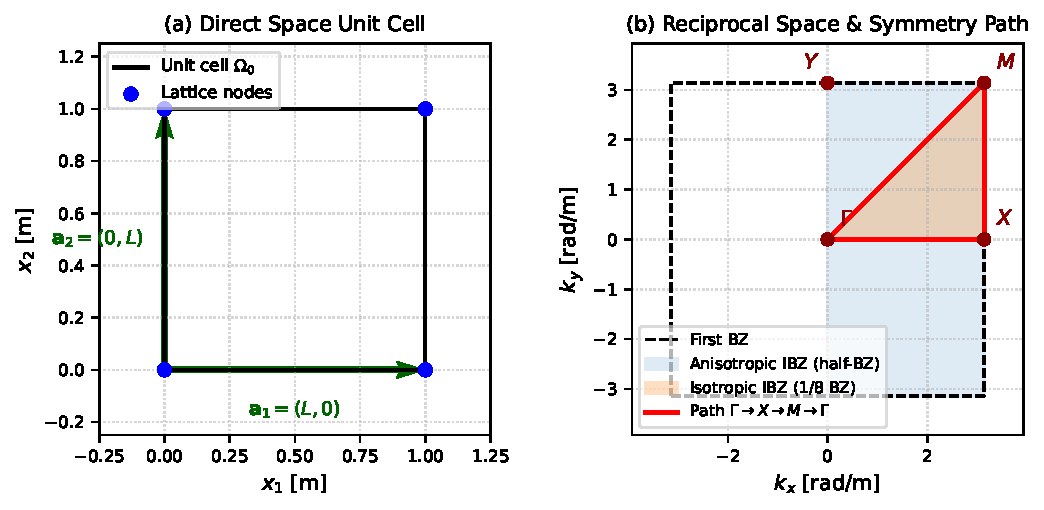
\includegraphics[width=\textwidth]{figures/fig02_lattice_ibz.pdf}
\caption{(a) Square periodic lattice. (b) First Brillouin zone and the high-symmetry contour $\Gamma$--$X$--$M$--$\Gamma$.}
\label{fig:lattice_ibz}
\end{figure}

For a time-harmonic displacement $\bmu(\bmx,t)=\tilde{\bmu}(\bmx)e^{\iu(\bmk\cdot\bmx-\omega t)}$, Bloch periodicity gives
\begin{equation}
\bmu(\bmx+\bm{a}_\alpha)=\bmu(\bmx)e^{\iu\bmk\cdot\bm{a}_\alpha},\qquad \alpha\in\{1,2\}.
\label{eq:bloch_displacement}
\end{equation}
Because the approximation is $C^1$-conforming, differentiating the displacement relation gives:
\begin{equation}
\begin{split}
\frac{\partial\bmu}{\partial x_\beta}(\bmx+\bm{a}_\alpha)&=\frac{\partial\bmu}{\partial x_\beta}(\bmx)e^{\iu\bmk\cdot\bm{a}_\alpha},\\
\frac{\partial^2\bmu}{\partial x_1\partial x_2}(\bmx+\bm{a}_\alpha)&=\frac{\partial^2\bmu}{\partial x_1\partial x_2}(\bmx)e^{\iu\bmk\cdot\bm{a}_\alpha}.
\end{split}
\label{eq:bloch_derivatives}
\end{equation}
Thus displacement, first derivatives, and cross derivatives all take the same Bloch phase; a different phase for derivative degrees of freedom would break $C^1$ continuity across cell boundaries.

\subsection{Nondimensionalization}
For Case~H, I scale length, frequency, and velocity with the cell length $L$, shear modulus $\mu$, and density $\rho$:
\begin{equation}
\begin{split}
\bark&=\frac{kL}{\pi},\qquad \barw=\frac{\omega}{\omega_0},\qquad
\omega_0=\sqrt{\frac{\mu}{\rho L^2}},\\
\bar{l}_m&=\frac{l_m}{L},\qquad
\ellbar=\frac{\ell_{\mathrm{i}}}{L},\qquad
\bar{v}_p=\frac{\omega/k}{\sqrt{\mu/\rho}}.
\end{split}
\label{eq:nondim_defs}
\end{equation}
This gives $c_T=1$ and $c_L=\sqrt{(\lambda+2\mu)/\mu}=\sqrt{3}$ for $\lambda/\mu=1$ ($\nu=0.25$). Case~C uses the matrix shear speed and frequency scale specified in Table~\ref{tab:case_params}.

\subsection{Gap and steering measures}
At each wave vector, the eigenfrequencies are ordered as $\barw_1(\bmk)\le\barw_2(\bmk)\le\cdots$. We distinguish gaps evaluated on one path leg, the complete high-symmetry path, and the full Brillouin zone:
\begin{enumerate}[label=(\alph*)]
  \item \textbf{Leg gap:} for bands $n$ and $n+1$, $\Delta[\mathrm{leg}]=\min_{\bmk\in\mathrm{leg}}\barw_{n+1}(\bmk)-\max_{\bmk\in\mathrm{leg}}\barw_n(\bmk)$; $\Delta_{GX}$ denotes the $\Gamma$--$X$ leg.
  \item \textbf{Path gap:}
  \begin{equation}
  \Delta_{\mathrm{path}}=\min_{\bmk\in\mathrm{path}}\barw_{n+1}(\bmk)-\max_{\bmk\in\mathrm{path}}\barw_n(\bmk).
  \label{eq:delta_path}
  \end{equation}
  \item \textbf{Complete gap:}
  \begin{equation}
  \Delta_{\mathrm{complete}}=\min_{\bmk\in\mathcal{B}}\barw_{n+1}(\bmk)-\max_{\bmk\in\mathcal{B}}\barw_n(\bmk).
  \label{eq:delta_complete}
  \end{equation}
\end{enumerate}
Since the leg, path, and full zone are nested sets, $\Delta[\mathrm{leg}]\ge\Delta[\mathrm{path}]\ge\Delta[\mathrm{complete}]$:
\begin{equation}
\Delta[\mathrm{leg}]\ge\Delta[\mathrm{path}]\ge\Delta[\mathrm{complete}].
\label{eq:gap_hierarchy}
\end{equation}
A positive leg gap indicates a directional spectral separation along that path; for a homogeneous, materially-uncontrasted cell such as Case~H this is a reduced-zone effect, not physical wave filtering. A complete band gap requires $\Delta_{\mathrm{complete}}>0$.

The orientation sensitivity of a directional gap is measured by
\begin{equation}
S_\theta=\frac{\max_\theta\left|\frac{\partial\Delta}{\partial\theta}\right|}{\max_\theta\Delta}\quad[\mathrm{rad}^{-1}].
\label{eq:S_theta_def}
\end{equation}
{\sloppy The angular derivative is evaluated on the sampled $15^\circ$ orientation grid $\theta\in\{0^\circ,15^\circ,\ldots,90^\circ\}$, using a central difference at interior points and a one-sided difference at the $\theta=0^\circ$ and $90^\circ$ endpoints.\par}

The group velocity and its angular deviation from the wave vector are
\begin{equation}
\bmv_g=\nabla_{\bmk}\omega.
\label{eq:group_velocity}
\end{equation}
\begin{equation}
\delta=\angle\bmv_g-\angle\bmk.
\label{eq:steering_angle}
\end{equation}

\section{$C^1$ Finite Element Discretisation}
\label{sec:fem}

\subsection{Bogner--Fox--Schmit Bicubic Hermite Element}
The Mindlin Form-II weak form contains second derivatives of displacement, so its trial functions must lie in the Sobolev space $H^2(\Omega)$. Standard $C^0$ Lagrange elements do not meet this conformity requirement. We use the Bogner--Fox--Schmit (BFS) bicubic element, which provides $C^1$ continuity across rectangular element boundaries on structured meshes \cite{bfs1965}.

For a rectangular element of dimensions $2a \times 2b$, I interpolate $u_1(x, y)$ and $u_2(x, y)$ independently, using tensor products of one-dimensional cubic Hermite polynomials:
\begin{equation}
u_i(x, y) = \sum_{a=1}^4 \sum_{p=1}^4 N_{a,p}(x, y) d_{i, a, p}^e, \quad i \in \{1, 2\},
\label{eq:bfs_interpolation}
\end{equation}
where $a \in \{1, 2, 3, 4\}$ indexes the four element vertices, and $p \in \{1, 2, 3, 4\}$ denotes the four nodal degrees of freedom per displacement component:
\begin{equation}
\bm{d}_{i, a}^e = \begin{bmatrix} u_i & \frac{\partial u_i}{\partial x} & \frac{\partial u_i}{\partial y} & \frac{\partial^2 u_i}{\partial x \partial y} \end{bmatrix}^\mathsf{T}_{\text{at node } a}.
\label{eq:nodal_dof_vector}
\end{equation}
With 4 vertices and 2 displacement components, each BFS element has $4 \times 2 \times 4 = 32$ degrees of freedom. Figure~\ref{fig:bfs_dof} shows the nodal DOFs and their Bloch-phase mapping at periodic boundaries. All reported band structures and design maps use a uniform mesh of $n \times n = 16 \times 16$ BFS elements per unit cell. This gives $h = L/n = 0.0625$ and $8 n^2 = 2048$ degrees of freedom per cell; Table~\ref{tab:case_params} lists the mesh size. Here $8n^2$ denotes the independent Bloch-reduced degrees of freedom, whereas the DOF counts reported in the supplementary Case-C resolution table (Table~S4) correspond to the assembled nodal system before Bloch reduction, $8(N+1)^2$.

\begin{figure}[htbp]
\centering
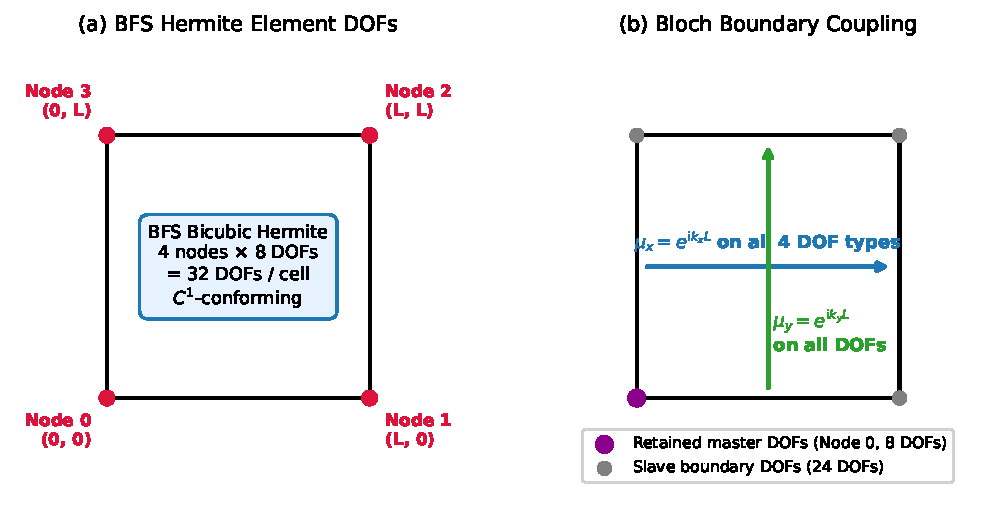
\includegraphics[width=\textwidth]{figures/fig03_bfs_dof_bloch.pdf}
\caption{(a) Nodal degrees of freedom in the 32-DOF $C^1$ Bogner--Fox--Schmit (BFS) element; each displacement component has 4 nodal DOFs, $\{u, u_{,x}, u_{,y}, u_{,xy}\}$. (b) Master--slave Bloch coupling at periodic boundaries. The phase $e^{\iu \bmk \cdot \bm{a}_\alpha}$ applies to displacement and derivative degrees of freedom alike.}
\label{fig:bfs_dof}
\end{figure}

\subsection{Element matrices}
The strain tensor $\bm\varepsilon$ and strain-gradient tensor $\bm\eta$ within element $e$ are related to the element nodal displacement vector $\bm{d}^e \in \mathbb{R}^{32}$ via kinematic strain-displacement matrices $\bmB^c$ and $\bmB^g_k$:
\begin{equation}
\bm\varepsilon = \bmB^c \bm{d}^e, \quad \bm\eta_k \equiv \frac{\partial \bm\varepsilon}{\partial x_k} = \bmB^g_k \bm{d}^e, \quad k \in \{1, 2\}.
\label{eq:strain_matrices}
\end{equation}
The element stiffness matrix $\bmK^e$ is the sum of classical and gradient contributions:
\begin{equation}
\bmK^e = \bmK^c + \bmK^g(\theta, \mathrm{AR}),
\label{eq:Ke_total}
\end{equation}
where the classical stiffness matrix is:
\begin{equation}
\bmK^c = \int_{\Omega_e} (\bmB^c)^\mathsf{T} \bmC \bmB^c \,\dif\Omega,
\label{eq:Kc_int}
\end{equation}
and the anisotropic gradient stiffness matrix is:
\begin{equation}
\bmK^g(\theta, \mathrm{AR}) = \frac{1}{10} \sum_{k=1}^2 \sum_{l=1}^2 L_{kl}(\theta) \int_{\Omega_e} (\bmB^g_k)^\mathsf{T} \bmC \bmB^g_l \,\dif\Omega.
\label{eq:Kg_int}
\end{equation}
Because the shape functions are bicubic tensor-product polynomials, each homogeneous-element stiffness and mass integrand has degree at most six in each coordinate. A four-point Gauss--Legendre rule is exact through degree seven, so the $4 \times 4$ tensor rule is the smallest rule that integrates all such terms exactly. This avoids quadrature error for homogeneous elements; the unconstrained stiffness still has its expected rigid-body null modes. In elements cut by the inclusion, the discontinuous material field is instead integrated by sub-cell Gauss sampling with an $O(h)$ geometric approximation (Section~\ref{sec:caseC_pc}).

\paragraph{Mass and micro-inertia matrices}
The kinetic energy gives the classical and micro-inertia mass contributions:
\begin{equation}
\bmM^e = \bmM_0 + \ell_{\mathrm{i}}^2 \bmM^g,
\label{eq:Me_total}
\end{equation}
with:
\begin{equation}
\begin{split}
\bmM_0 &= \rho \int_{\Omega_e} \bm{N}^\mathsf{T} \bm{N} \,\dif\Omega, \\
\bmM^g &= \rho \sum_{k=1}^2 \int_{\Omega_e} \left(\frac{\partial \bm{N}}{\partial x_k}\right)^\mathsf{T} \left(\frac{\partial \bm{N}}{\partial x_k}\right) \,\dif\Omega.
\end{split}
\label{eq:Mg_int}
\end{equation}
Both $\bmM_0$ and $\bmM^g$ are symmetric and positive semi-definite; their sum $\bmM^e$ is strictly positive definite for any positive density $\rho > 0$.

\subsection{Bloch reduction and eigenproblem}
We partition the global degrees of freedom $\bm{d}$ into interior ($I$), master-boundary ($M$), and slave-boundary ($S$) sets to impose the Bloch conditions on $\partial\Omega_{\mathrm{cell}}$:
\begin{equation}
\bm{d} = \begin{bmatrix} \bm{d}_I \\ \bm{d}_M \\ \bm{d}_S \end{bmatrix}.
\label{eq:d_partition}
\end{equation}
The Bloch transformation relates the slave DOFs on the top and right boundaries to the corresponding master DOFs on the bottom and left boundaries:
\begin{equation}
\bm{d}_S = \bmT_{SM}(\bmk) \bm{d}_M,
\label{eq:slave_master_rel}
\end{equation}
where $\bmT_{SM}(\bmk)$ is a diagonal complex phase matrix formed by evaluating $e^{\iu k_x L}$, $e^{\iu k_y L}$, or $e^{\iu (k_x + k_y)L}$ for each periodic node pair. As derived in Section~\ref{sec:bloch}, identical phase factors apply to the displacement, first-order, and cross-derivative DOFs.

In the continuous weak form, natural boundary work cancels between opposite cell faces. The effective traction $p_i^{\mathrm{dyn}}$ defined in Section~\ref{sec:continuum} carries the Bloch phase and changes sign with the outward normal; its test trace carries the conjugate phase. The double traction $R_i=n_jn_k\tau_{ijk}$ also carries the Bloch phase but is unchanged when the normal reverses, while its work-conjugate normal derivative changes sign. These signs and phases cancel both face integrals. Line and corner terms pair under the same translations, including the product phase $e^{\iu(k_x+k_y)L}$ at the corner; no separate free-boundary condition is imposed on a Bloch-paired face.

We collect these relations in the master--slave transformation matrix $\bmT(\bmk)$:
\begin{equation}
\bm{d} = \bmT(\bmk) \bar{\bm{d}}, \quad \bmT(\bmk) = \begin{bmatrix} \mathbf{I}_{II} & \mathbf{0} \\ \mathbf{0} & \mathbf{I}_{MM} \\ \mathbf{0} & \bmT_{SM}(\bmk) \end{bmatrix}, \quad \bar{\bm{d}} = \begin{bmatrix} \bm{d}_I \\ \bm{d}_M \end{bmatrix},
\label{eq:T_bloch}
\end{equation}
The reduced stiffness and mass matrices follow from Galerkin projection:
\begin{equation}
\bar{\bmK}(\bmk) = \bmT(\bmk)^\mathsf{H} \bmK \bmT(\bmk), \quad \bar{\bmM}(\bmk) = \bmT(\bmk)^\mathsf{H} \bmM \bmT(\bmk).
\label{eq:reduced_KM}
\end{equation}

\paragraph{Reduced Hermitian eigenproblem}
We obtain the dispersion curves $\barw_n(\bmk)$ from the reduced generalized eigenvalue problem:
\begin{equation}
\left[ \bar{\bmK}(\bmk) - \omega^2 \bar{\bmM}(\bmk) \right] \bar{\bm{d}} = \bm{0}.
\label{eq:eigenproblem}
\end{equation}
Each entry of the diagonal phase subblock $\bmT_{SM}(\bmk)$ has unit modulus, so this subblock is unitary. The full map $\bmT(\bmk)$ is rectangular and full-column-rank, but is not unitary. For positive elastic and inertial parameters, the full-cell matrices satisfy $\bmK\succeq 0$ and $\bmM\succ 0$; the reduced operators are therefore Hermitian:
\begin{equation}
\bar{\bmK}(\bmk)^\mathsf{H} = \bar{\bmK}(\bmk) \succeq 0, \quad \bar{\bmM}(\bmk)^\mathsf{H} = \bar{\bmM}(\bmk) \succ 0,
\label{eq:hermiticity}
\end{equation}
The generalized eigenvalues $\omega_n^2$ are therefore real and nonnegative. Shifting $\bmk$ by a reciprocal-lattice vector $\bm{G}$ leaves every Bloch phase unchanged, so the reduced stiffness and mass matrices satisfy $\bar{\bmK}(\bmk + \bm{G}) = \bar{\bmK}(\bmk)$ and $\bar{\bmM}(\bmk + \bm{G}) = \bar{\bmM}(\bmk)$. The spectrum is periodic across reciprocal space.

\paragraph{Branch tracking}
Modes with different spatial symmetries can cross along high-symmetry paths. We track their identity between adjacent wave vectors using the Modal Assurance Criterion (MAC) at $\bmk_1$ and $\bmk_2$. Let $\bm{d}_m(\bmk)=\bmT(\bmk)\bar{\bm{d}}_m(\bmk)$ be the corresponding full-cell eigenvector, and let $\bmM$ be the common, assembled full-cell mass matrix, including gradient micro-inertia. The cross-wavevector MAC is
\begin{equation}
\mathrm{MAC}_{mn}(\bmk_1,\bmk_2) = \frac{\left| \bm{d}_m(\bmk_1)^\mathsf{H} \bmM \bm{d}_n(\bmk_2) \right|^2}{\left( \bm{d}_m(\bmk_1)^\mathsf{H} \bmM \bm{d}_m(\bmk_1) \right) \left( \bm{d}_n(\bmk_2)^\mathsf{H} \bmM \bm{d}_n(\bmk_2) \right)}
\label{eq:mac_def}
\end{equation}
The lifted vectors use a common full-cell mass metric; the reduced mass matrix depends on $\bmk$ and is not used to compare modes at different wave vectors. If the off-diagonal MAC indicates a branch exchange, the continuation step is halved. Band gaps are computed from the frequency-ordered eigenvalues $\barw_1(\bmk) \le \barw_2(\bmk) \le \dots \le \barw_N(\bmk)$, independently of the mode labels assigned during tracking.

\section{Verification and numerical resolution}
\label{sec:verification}

We compare the implementation with analytical limits, independent transfer-matrix calculations, algebraic identities, and mesh-refinement results. For the published heterogeneous bilayers only graphical agreement is available, and cases with ambiguous parameters or no numerical curves are not treated as external validation.

\subsection{Analytical limits and bilayer comparison}
In the isotropic homogeneous limit, the long-wavelength phase velocities recover the classical transverse and longitudinal speeds:
\begin{equation}
\begin{split}
\lim_{k\to0}\frac{\omega_T(k)}{k}&=\sqrt{\frac{\mu}{\rho}}=1.0,\\
\lim_{k\to0}\frac{\omega_L(k)}{k}&=\sqrt{\frac{\lambda+2\mu}{\rho}}=\sqrt{3}\approx1.73205.
\end{split}
\label{eq:acoustic_limits}
\end{equation}
At $\bar{k}=0.001$, the computed acoustic speeds differ from these limits by $1.25\times10^{-8}$ (Table~\ref{tab:consistency_suite}). The pure-bending micro-beam reduction matches the published closed-form limits to within $10^{-15}$ \cite{papargyribeskou2009}; details appear in the supplementary material (Sec.~S2). The micro-inertia asymptote is checked separately in Appendix~\ref{app:asymptotics} and Section~\ref{sec:microinertia}.

As a classical reference, I analyze a periodic AlN/BaTiO$_3$ bilayer with $a_A=a_B=0.01\,\mathrm{m}$ and $b=a_A+a_B=0.02\,\mathrm{m}$ using the Rytov relation \cite{li2024anchorB,zhengwei2009}:
\begin{equation}
\begin{split}
\cos(Kb)={}&\cos(k_Aa_A)\cos(k_Ba_B) \\
&-\frac{1}{2}\left(\frac{Z_A}{Z_B}+\frac{Z_B}{Z_A}\right)\sin(k_Aa_A)\sin(k_Ba_B),
\end{split}
\label{eq:rytov}
\end{equation}
where $k_m=\omega\sqrt{\rho_m/c_{33,m}}$, $v_m=\sqrt{c_{33,m}/\rho_m}$, and $Z_m=\rho_m v_m$. The single-layer transfer-matrix identity and the identical-material bilayer reduction match their analytical limits to $6.47\times10^{-16}$ and $7.22\times10^{-16}$, respectively. The heterogeneous transfer-matrix trace reproduces the Rytov relation to $2.22\times10^{-16}$. The first three calculated stop-band intervals are $[0.4806,0.5209]$, $[0.9812,1.0215]$, and $[1.4993,1.5028]$ in normalized frequency. We compare the result with the published B1 plot visually because tabulated source data are unavailable; no percentage error is inferred from the curves.

We reproduce two gradient-elastic bilayer cases, but do not treat them as external validations. One published length-scale definition is dimensionally ambiguous. For the other, the plotted parameter set and normalization are unspecified, and the numerical curves are unavailable. The supplementary material (Sec.~S2) records these limitations and the status of each comparison. We also compare the dipolar layer matrix with the source's printed formulation; this checks the formulation but does not validate its band curves.

\subsection{Numerical consistency and mesh convergence}
The consistency checks assess operator Hermiticity, Brillouin-zone periodicity, isotropic rotational invariance, acoustic slopes, rotation--swap symmetry, matrix definiteness, the micro-inertia limit, and the energy-flux/group-velocity identity; Table~\ref{tab:consistency_suite} lists the results. The energy-flux identity is evaluated on closed-form Case-H harmonic fields with the sign convention of Appendix~\ref{app:energy_flux}, comparing the cycle-averaged energy flux with a central-difference group velocity for the transverse and longitudinal acoustic branches along several in-plane directions; it holds to $6.91\times10^{-10}$. The supplementary material (Sec.~S3) gives the check definitions and expanded diagnostics.

We assess mesh convergence for homogeneous Case~H on uniform $n\times n$ BFS grids, $n\in\{4,8,16,32\}$, at fixed $\bmk=(0.31\pi/L,0.22\pi/L)$. Figure~\ref{fig:mesh_convergence} shows the acoustic-frequency error relative to the closed-form value and the change between successive meshes. The fitted empirical rate is $p=4.17$ (95\% CI $[3.15,5.20]$) over the $4^2$, $8^2$, and $16^2$ levels. The reported $32^2$ result is resolution-limited and is excluded from the fit. This rate is empirical; it is not a theoretical-order claim. The operational mesh-change floor is $\varepsilon_\Delta=4.63\times10^{-11}$ and is distinct from eigensolver reproducibility. The smallest positive sampled directional separation across the 42-configuration design map, $\Delta_{GX}=1.3\times10^{-3}$ (at $\mathrm{AR}=5$, $\theta=0^\circ$; see Table~\ref{tab:gap_summary}), exceeds the floor by approximately $3\times10^7$.

\begin{figure*}[htbp]
\centering
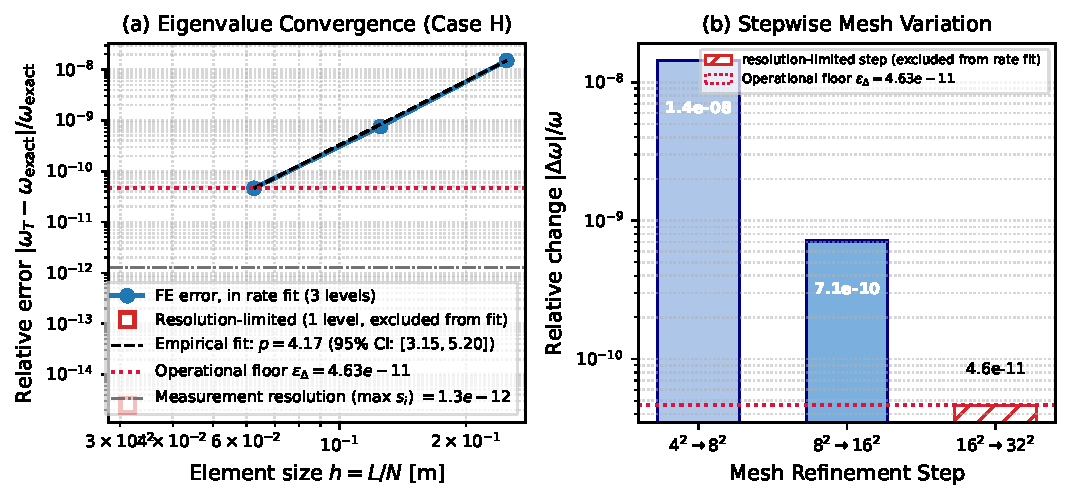
\includegraphics[width=\textwidth]{figures/fig05_mesh_convergence.pdf}
\caption{Case-H mesh study for the acoustic branch. (a) Relative frequency error versus element size; the $32^2$ result is shown as resolution-limited and is not included in the empirical fit. (b) Successive-mesh change and the operational mesh-change floor $\varepsilon_\Delta$}
\label{fig:mesh_convergence}
\end{figure*}

\begin{table*}[htbp]
\begin{center}
\begin{threeparttable}
\tablebodyfont
\caption{Analytical and numerical consistency checks. All rows except the energy-flux identity assess the Bloch finite-element implementation directly; the energy-flux identity is a closed-form continuum check evaluated on exact Case-H harmonic fields (see text), not a check of the finite-element eigenvectors}
\label{tab:consistency_suite}
\small
\begin{tabular}{@{}p{2.3cm} p{6.9cm} p{2.2cm} c p{1.8cm}@{}}
\toprule
Check & Quantity assessed & Maximum discrepancy & Criterion & Result \\
\midrule
Hermiticity & Reduced stiffness and mass operators & $2.01\times10^{-16}$; $5.63\times10^{-17}$ & $<10^{-12}$ & Within criterion \\
Brillouin-zone periodicity & Spectrum under reciprocal-lattice shifts & $9.66\times10^{-16}$ & $<10^{-10}$ & Within criterion \\
Isotropic rotation & Frequencies at $\mathrm{AR}=1$ & $9.63\times10^{-16}$ & $<10^{-10}$ & Within criterion \\
Acoustic limit & Long-wave transverse and longitudinal slopes & $1.25\times10^{-8}$ & $<10^{-6}$ & Within criterion \\
Rotation--swap symmetry & Spectrum under $\theta\mapsto\theta+90^\circ$ and axis swap & $6.44\times10^{-16}$ & $<10^{-10}$ & Within criterion \\
Definiteness & Two rigid modes at $\Gamma$; positive interior spectrum & As expected & Admissible & As expected \\
Micro-inertia limit & Phase speed at $\bar{k}=200$ versus asymptotic value & $2.85\times10^{-4}$ & $<10^{-3}$ & Within criterion \\
Energy-flux identity (closed-form) & Closed-form group velocity versus cycle-averaged energy flux, Case-H harmonic fields & $6.91\times10^{-10}$ & $<10^{-6}$ & Within criterion \\
\bottomrule
\end{tabular}

\end{threeparttable}
\end{center}
\end{table*}

Selected Case-H and Case-C inputs appear in Table~\ref{tab:case_params}. The supplementary material (Secs.~S1--S4) contains the full parameter summary, external-comparison details, and extended convergence diagnostics.

\section{Results: dispersion, band gaps, and wave steering}
\label{sec:results}

We begin from the homogeneous isotropic reference and trace the effect of the length tensor on the dispersion branches, on the directional spectral separation and on its sampled design map, then turn to the heterogeneous Case~C and to group-velocity steering; Section~\ref{sec:microinertia} treats the high-wavenumber response. Case~H is a homogeneous medium analyzed on a periodic cell that carries no material contrast, so a positive $\Delta_{GX}$ is a reduced-zone spectral separation of that medium and not a Bragg attenuation gap of a physically periodic one. Case~C does carry periodic contrast and therefore supports a genuine complete band gap. Unless otherwise stated, every reported Case-H directional and complete-gap measure ($\Delta_{GX}$, $\Delta_{XM}$, $\Delta_{MG}$, $\Delta_{\mathrm{path}}$, $\Delta_{\mathrm{complete}}$) is evaluated on the Bands~2--3 pair. Table~\ref{tab:case_params} lists selected inputs and Supplementary Material~S1 the full parameter set.

\begin{table}[htbp]
\centering
\caption{Selected material and numerical inputs for Cases H and C and the steering analysis.}
\label{tab:case_params}
\begin{tabular}{@{}l p{2.9cm} p{10.8cm}@{}}
\toprule
Case & Quantity & Value \\
\midrule
H & Cell and matrix & $L=1.0\,\mathrm{m}$; $\lambda=\mu=1.0\,\mathrm{Pa}$; $\rho=1.0\,\mathrm{kg/m^3}$ \\
H & Lengths and mesh & $l_{\mathrm{iso}}=0.20\,\mathrm{m}$; $\ell_{\mathrm{i}}=0.20\,\mathrm{m}$; $16\times16$ BFS elements per cell \\
C & Epoxy matrix & $\rho_m=1142\,\mathrm{kg/m^3}$; $\mu_m=1.48\,\mathrm{GPa}$; $\lambda_m=4.57\,\mathrm{GPa}$ \\
C & YBCO inclusion & $\rho_i=6333\,\mathrm{kg/m^3}$; $\mu_i=37.0\,\mathrm{GPa}$; $\lambda_i=95.0\,\mathrm{GPa}$ \\
C & Geometry and length scales & $L=1.0\,\mathrm{m}$; $r_0/L=0.30$; $\ell_m/L=0.10$; $\ell_i/L=0.20$ \\
C & Frequency scale and reported resolution & $c_{t,m}=1138.4\,\mathrm{m/s}$; $\omega_{0,C}=\pi c_{t,m}/L=3576.4\,\mathrm{rad/s}$; $4\times4$ mesh and $21\times21$ zone grid \\
Steering & Acoustic-branch sweep & $\bar{k}=0.5$; $\mathrm{AR}\in\{5,10\}$; $\theta=0^\circ,15^\circ,\ldots,90^\circ$ \\
\bottomrule
\end{tabular}

\end{table}

\subsection{Homogeneous isotropic baseline}
At $\mathrm{AR}=1$, the principal characteristic lengths coincide and the rotated length tensor is isotropic, so its constitutive response is independent of $\theta$. It therefore provides the reference for the anisotropic calculations, and Figure~\ref{fig:caseH_dispersion} plots its branches alongside theirs; its $\Gamma$--$X$ directional width is $\Delta_{GX}=0.041$.

\subsection{Anisotropy reshapes the Case-H branches}
Figure~\ref{fig:caseH_dispersion} compares the isotropic reference with two orientations of the anisotropic length tensor. Both acoustic branches start at zero frequency at $\Gamma$. Changing aspect ratio and orientation shifts the branches and lifts symmetry-related degeneracies at the zone edge. At $\mathrm{AR}=10$ and $\theta=45^\circ$, a narrow reduced-zone spectral separation appears along $\Gamma$--$X$, with $\Delta_{GX}=0.0043$. Modes propagating in other directions overlap this interval, so it is not a complete gap; the full-zone measure remains $\Delta_{\mathrm{complete}}\le -0.3235$.

In this model, the rotated length tensor changes the gradient-stiffness contribution according to propagation direction. The resulting branch shifts are therefore not uniform across the Brillouin zone: adjacent bands can separate along $\Gamma$--$X$ while modes at other wave vectors remain in the same frequency interval.

\begin{figure}[htbp]
\centering
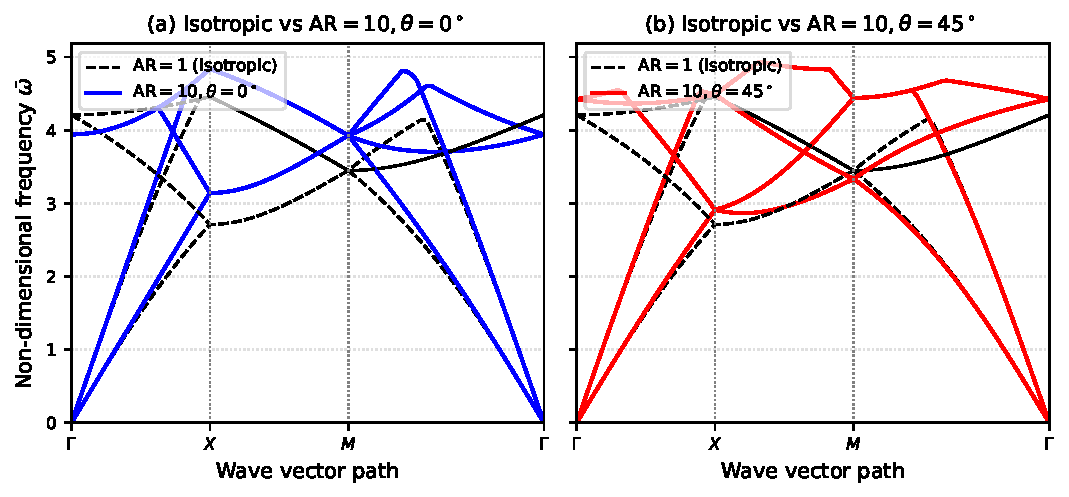
\includegraphics[width=\textwidth]{figures/fig06_caseH_dispersion.pdf}
\caption{Case-H Bloch bands along $\Gamma$--$X$--$M$--$\Gamma$. (a) Isotropic reference ($\mathrm{AR}=1$) and aligned anisotropy ($\mathrm{AR}=10$, $\theta=0^\circ$). (b) Isotropic reference and diagonal anisotropy ($\mathrm{AR}=10$, $\theta=45^\circ$), which opens a narrow $\Gamma$--$X$ reduced-zone spectral separation but no complete gap.}
\label{fig:caseH_dispersion}
\end{figure}

\subsection{Aspect-ratio and orientation effects}
Figure~\ref{fig:theta_sweep} shows the zone-edge frequencies as the tensor rotates. At $\mathrm{AR}=5$, as $\theta$ changes from $0^\circ$ to $90^\circ$, the transverse and longitudinal frequencies at $X$ fall from $2.915$ to $2.672$ and from $5.050$ to $4.628$, respectively, as the projected length scale shifts from the major to the minor axis. The $M$-point frequencies are symmetric about $45^\circ$, as expected from the square-cell symmetry.

\begin{figure}[htbp]
\centering
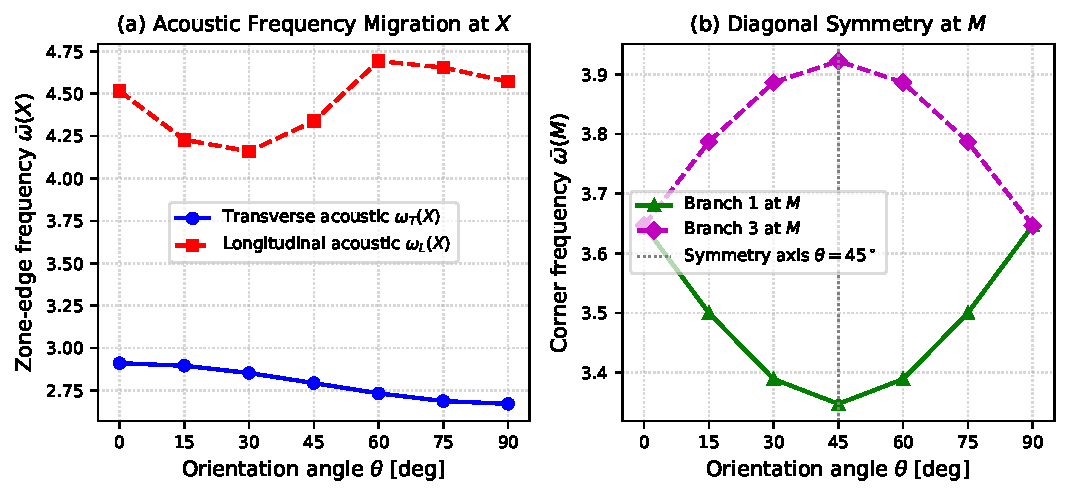
\includegraphics[width=\textwidth]{figures/fig08_theta_sweep.pdf}
\caption{Orientation dependence of the first four Case-H eigenfrequencies at (a) $X$ and (b) $M$ for $\mathrm{AR}=5$. The $M$-point response is symmetric about $\theta=45^\circ$.}
\label{fig:theta_sweep}
\end{figure}

Figure~\ref{fig:ar_sweep} isolates elongation at fixed $\theta=45^\circ$, using volume-equivalent length scaling. Increasing $\mathrm{AR}$ lengthens the major characteristic length while shortening the minor one, so the directional gradient-stiffness contribution and the two bounding band edges need not shift together. Because the gap width is their frequency difference, it can vary non-monotonically even when an individual branch moves consistently.

\begin{figure}[htbp]
\centering
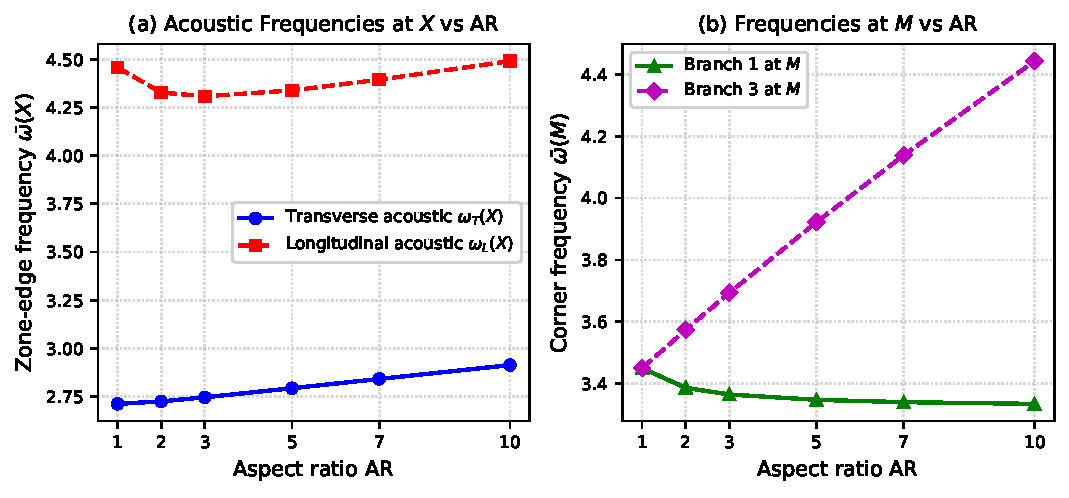
\includegraphics[width=\textwidth]{figures/fig09_ar_sweep.pdf}
\caption{Case-H branch frequencies at $X$ and $M$ as the aspect ratio varies from $1$ to $10$ at fixed $\theta=45^\circ$, using volume-equivalent length scaling.}
\label{fig:ar_sweep}
\end{figure}

\subsection{Directional spectral separation}
A positive $\Delta_{GX}$ marks a separation on the $\Gamma$--$X$ leg only: modes at other wave vectors still occupy the same frequency interval. The $\mathrm{AR}=10$, $\theta=45^\circ$ configuration makes the point, with $\Delta_{GX}=0.0043$ against a negative complete-gap measure, and every homogeneous configuration listed behaves the same way. Table~\ref{tab:gap_summary} reports the representative directional and complete-gap measures; Supplementary Material~S3 gives normalized widths and mesh-to-mesh variations.

\subsection{Design-map interpretation}
Across the 42 evaluated $(\theta,\mathrm{AR})$ configurations in Figure~\ref{fig:design_map}, the largest sampled $\Delta_{GX}=0.0677$ occurs at $(0^\circ,7)$. The response is non-monotone in aspect ratio. The plotted surface interpolates the evaluated points rather than a continuous optimum, and Figure~\ref{fig:polar_map} classifies the same samples by the sign of $\Delta_{GX}$. The orientation sensitivity $S_\theta$ is largest at $\mathrm{AR}=10$ ($2.34\,\mathrm{rad}^{-1}$).

\begin{figure}[htbp]
\centering
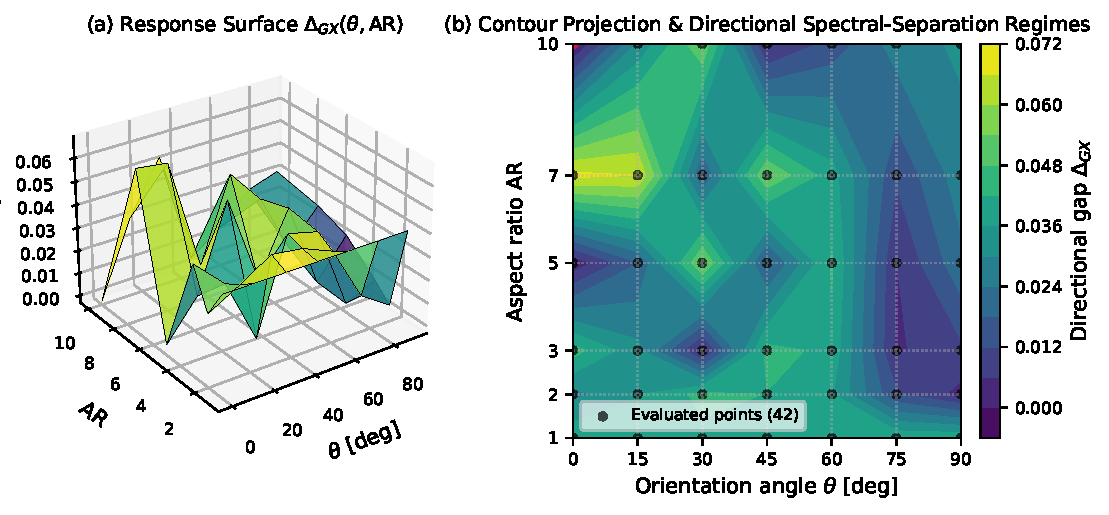
\includegraphics[width=\textwidth]{figures/fig10_design_map_3d.pdf}
\caption{Sampled Case-H design response $\Delta_{GX}(\theta,\mathrm{AR})$ for 42 configurations. The largest sampled value is $0.0677$ at $\theta=0^\circ$, $\mathrm{AR}=7$; at $\theta=45^\circ$, $\mathrm{AR}=10$, $\Delta_{GX}=0.0043$.}
\label{fig:design_map}
\end{figure}

\begin{figure}[htbp]
\centering
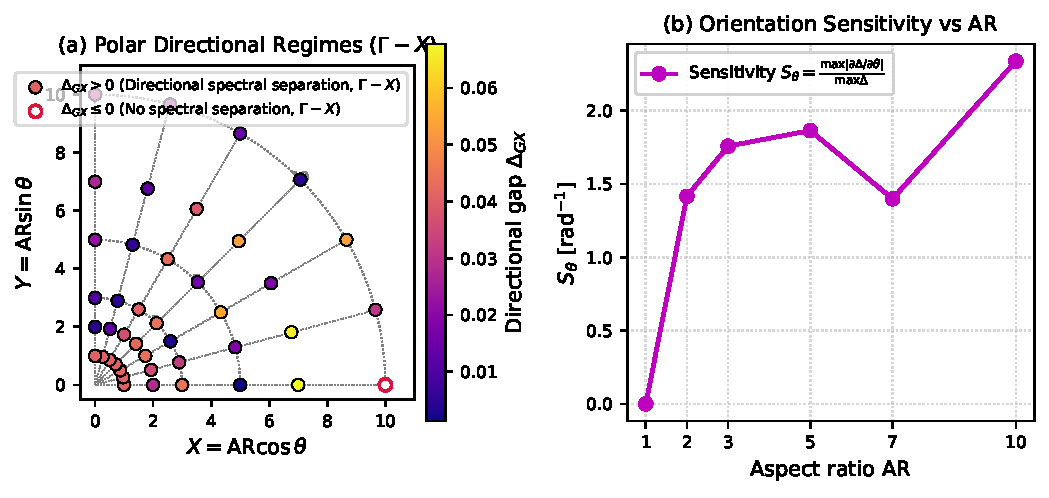
\includegraphics[width=\textwidth]{figures/fig11_polar_map_regimes.pdf}
\caption{Polar-coordinate view of the sampled Case-H designs, classified by $\Delta_{GX}\le0$ (pass band) and $\Delta_{GX}>0$ (directional spectral separation). The displayed boundary is a visual summary of sampled points.}
\label{fig:polar_map}
\end{figure}

\begin{table}[htbp]
\centering
\caption{Directional and complete-gap measures for representative Case-H configurations; values are reported at the precision retained between the $8\times8$ and $16\times16$ meshes.}
\label{tab:gap_summary}
\begin{tabular}{@{}c c r r r@{}}
\toprule
$\mathrm{AR}$ & $\theta$ & $\Delta_{GX}$ & $\Delta_{\mathrm{path}}$ & $\Delta_{\mathrm{complete}}$ \\
\midrule
$1$ & $0^\circ$  & $+0.041$ & $-0.32$ & $-0.32$ \\
$1$ & $45^\circ$ & $+0.041$ & $-0.32$ & $-0.32$ \\
$1$ & $90^\circ$ & $+0.041$ & $-0.32$ & $-0.32$ \\
$3$ & $0^\circ$  & $+0.045$ & $-0.10$ & $-0.46$ \\
$3$ & $45^\circ$ & $+0.044$ & $-0.45$ & $-0.48$ \\
$3$ & $90^\circ$ & $+0.011$ & $-0.33$ & $-0.46$ \\
$5$ & $0^\circ$  & $+0.001$ & $-0.01$ & $-0.58$ \\
$5$ & $45^\circ$ & $+0.016$ & $-0.48$ & $-0.58$ \\
$5$ & $90^\circ$ & $+0.022$ & $-0.37$ & $-0.58$ \\
$10$ & $0^\circ$  & $-0.002$ & $-0.24$ & $-0.85$ \\
$10$ & $45^\circ$ & $+0.004$ & $-0.29$ & $-0.56$ \\
$10$ & $90^\circ$ & $+0.031$ & $-0.65$ & $-0.85$ \\
\bottomrule
\end{tabular}
\footnotetext{$S_\theta$ [rad$^{-1}$]: AR $=1$: $0.00$; $2$: $1.42$; $3$: $1.76$; $5$: $1.86$; $7$: $1.40$; $10$: $2.34$.}

\end{table}

\subsection{Heterogeneous Case C: complete gap with periodic contrast}
\label{sec:caseC_pc}
Case~C combines gradient elasticity with a periodic epoxy--YBCO impedance contrast ($\chi_\mu=25.0$, $\chi_\rho=5.546$; Table~\ref{tab:case_params}), unlike homogeneous Case~H. We denote the cell period by $L$ in the text and $a$ in Figure~\ref{fig:caseC_dispersion}; $r_0/L=r_0/a=0.30$ gives a filling fraction of $28.27\%$. The circular interface is integrated by sub-cell Gauss sampling on the Cartesian mesh. Figure~\ref{fig:caseC_dispersion} shows a complete gap between Bands~3 and~4 over $\bar{\omega}\in[4.5698,7.1430]$. On the $4\times4$ mesh and $21\times21$ Brillouin-zone grid, $\Delta_{\mathrm{complete}}=2.5732$, or $43.94\%$. Brillouin-zone refinement changes the quoted width by less than $4\times10^{-4}$; finite-element refinement has a much larger effect.

\begin{figure}[htbp]
\centering
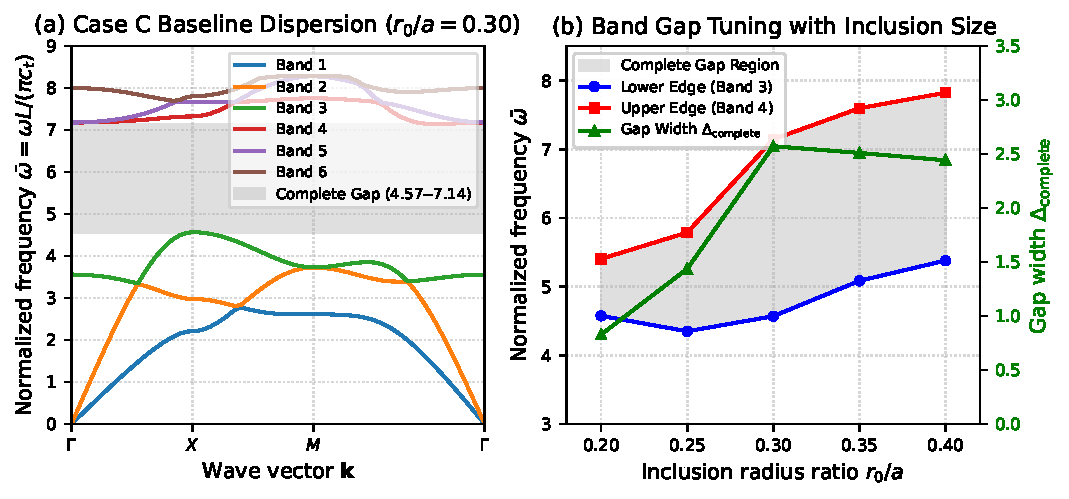
\includegraphics[width=\textwidth]{figures/fig07_caseC_dispersion.pdf}
\caption{Case-C complete-gap formation and radius dependence. (a) Bands along $\Gamma$--$X$--$M$--$\Gamma$ for $r_0/L=0.30$, with the $4\times4$-mesh gap between Bands~3 and~4. (b) Complete-gap width versus $r_0/a$ at the same mesh; the $r_0/a=0.30$ result is not mesh-converged.}
\label{fig:caseC_dispersion}
\end{figure}

Under mesh refinement, the complete gap falls from $2.5732$ at $4\times4$ to $2.2504$, $2.0722$, $1.9736$, and $1.9179$ at $8\times8$, $16\times16$, $32\times32$, and $64\times64$, respectively. It stays open at every computed resolution but has not converged. The value $2.5732$ is therefore a coarse-mesh result, not a continuum estimate. At the $4\times4$ mesh, increasing $r_0/L$ from $0.20$ to $0.30$ widens the gap from $0.8288$ ($16.61\%$) to $2.5732$ ($43.94\%$); it then narrows to $2.4426$ ($37.00\%$) at $r_0/L=0.40$. Supplementary Material~S4 gives the mesh, quadrature, and zone-sampling details.

\subsection{Group-velocity steering}
\label{sec:steering}
On the constant-wavenumber ring $|\bmk|=\bar{k}=0.5$, anisotropy makes the group velocity non-collinear with the wave vector. Since $\bmv_g=\nabla_{\bmk}\omega$ is normal to the local constant-frequency contours, their slope determines the angular departure of $\bmv_g$ from $\bmk$. Figure~\ref{fig:ifc_wave_steering} plots the angular deviation $\delta(\phi)=\angle\bmv_g-\angle\bmk$ and group-velocity magnitude at $\theta=45^\circ$. The peak deviation rises from $0^\circ$ at $\mathrm{AR}=1$ to $1.4146^\circ$ at $\mathrm{AR}=5$ and $2.7846^\circ$ at $\mathrm{AR}=10$. The magnitude $|\bmv_g|$ also varies around the contour, so the anisotropic dispersion changes the energy-transport speed as well as its direction.

\begin{figure}[htbp]
\centering
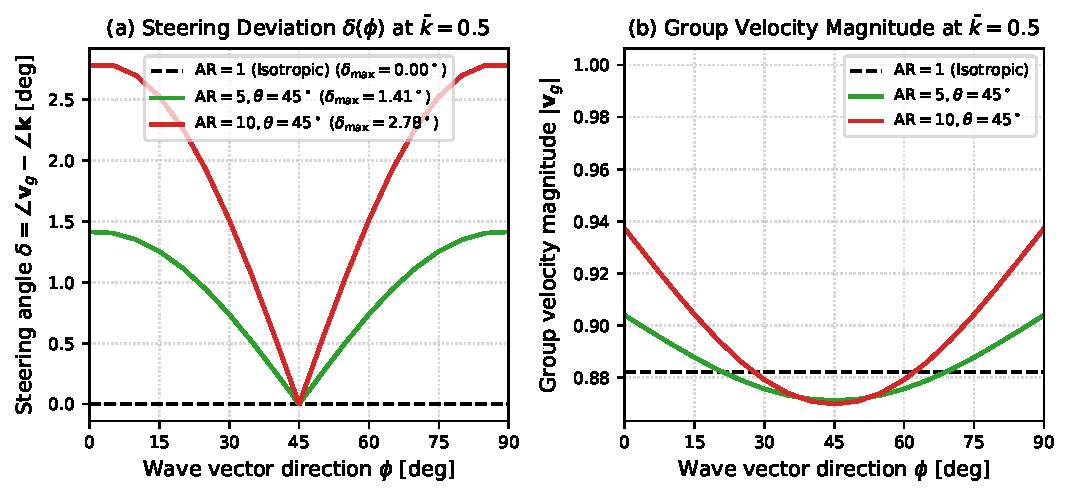
\includegraphics[width=\textwidth]{figures/fig12_ifc_wave_steering.pdf}
\caption{Acoustic-branch group-velocity steering on $|\bmk|=0.5$ at $\theta=45^\circ$. (a) Angular deviation for $\mathrm{AR}=1,5,10$, with peak values $0^\circ$, $1.4146^\circ$, and $2.7846^\circ$. (b) Directional variation of group-velocity magnitude.}
\label{fig:ifc_wave_steering}
\end{figure}

Figure~\ref{fig:s7_steering_sweep} and Table~\ref{tab:steering_sweep} report the orientation sweep $\theta\in\{0^\circ,15^\circ,\ldots,90^\circ\}$ for $\mathrm{AR}=5$ and $10$ on the same ring and acoustic branch, with the ring sampled at $5^\circ$ resolution and the reported peak refined by parabolic interpolation about the sampled maximum. Across the sampled orientations, the refined peak deviation varies by less than $10^{-5}\,$deg about $1.4146^\circ$ and $2.7846^\circ$, respectively; this measures the numerical invariance of the refinement procedure, not a $10^{-5}$-degree physical angular accuracy. The principal direction follows $\phi^*(\theta)\simeq(45^\circ-\theta)\bmod90^\circ$; at $\mathrm{AR}=10$, its excursions are at most $5^\circ$. These samples show that rotating the tensor repositions the steering lobes while leaving the peak angular deviation nearly unchanged; for this branch and ring, orientation chiefly redirects the group-velocity/energy-flow direction ($\bmv_g=\nabla_{\bmk}\omega$) rather than increasing its sampled maximum.

\begin{figure}[htbp]
\centering
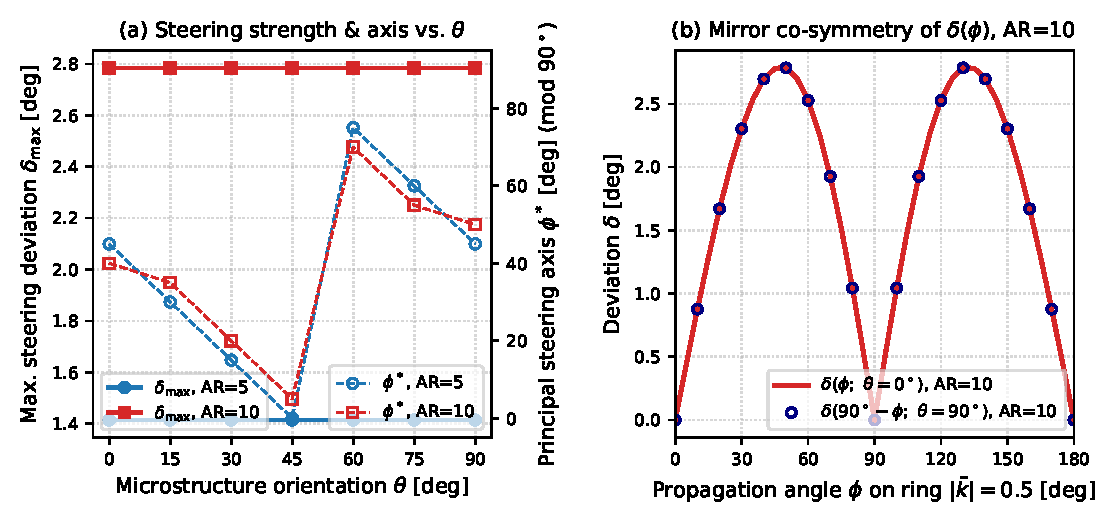
\includegraphics[width=\textwidth]{figures/fig14_s7_steering_sweep.pdf}
\caption{Orientation dependence of steering on $|\bmk|=0.5$. (a) Peak deviation $\delta_{\max}$ and principal direction $\phi^*$ for $\mathrm{AR}=5,10$; the peak angular deviation is invariant over the sampled orientations, while the lobe direction follows the rotated tensor axes on the $5^\circ$ ring grid. (b) The $\theta=0^\circ$ and $90^\circ$ deviation fields at $\mathrm{AR}=10$ exhibit mirror co-symmetry.}
\label{fig:s7_steering_sweep}
\end{figure}

\begin{table}[htbp]
\centering
\caption{Peak group-velocity deviation and principal steering direction across the sampled orientations at $\bar{k}=0.5$.}
\label{tab:steering_sweep}
\setlength{\tabcolsep}{4.5pt}%
\begin{tabular}{@{}c r r r r@{}}
\toprule
$\theta$ & \multicolumn{2}{c}{$\mathrm{AR}=5$} & \multicolumn{2}{c}{$\mathrm{AR}=10$} \\
\cmidrule(lr){2-3}\cmidrule(lr){4-5}
 & $\delta_{\max}$ [deg] & $\phi^*$ [deg] & $\delta_{\max}$ [deg] & $\phi^*$ [deg] \\
\midrule
$0^\circ$ & 1.4146 & 45 & 2.7846 & 40 \\
$15^\circ$ & 1.4146 & 30 & 2.7846 & 35 \\
$30^\circ$ & 1.4146 & 15 & 2.7846 & 20 \\
$45^\circ$ & 1.4146 & 0 & 2.7846 & 5 \\
$60^\circ$ & 1.4146 & 75 & 2.7846 & 70 \\
$75^\circ$ & 1.4146 & 60 & 2.7846 & 55 \\
$90^\circ$ & 1.4146 & 45 & 2.7846 & 50 \\
\bottomrule
\end{tabular}
\footnotetext{$M_s=\phi^*(90^\circ)-\phi^*(0^\circ)$: $M_s(\mathrm{AR}=5)=0^\circ$ and $M_s(\mathrm{AR}=10)=10^\circ$. The $5^\circ$ ring-sampling step limits the resolution of this difference; parabolic peak refinement remains within one sampling step.}
\footnotetext{Headless periodicity and mirror co-symmetry residuals are each $\le1.3\times10^{-6}\,$deg: $\delta(\phi;\theta)=\delta(\phi+180^\circ;\theta)$ and $\delta(\phi;\theta)=\delta(90^\circ-\phi;90^\circ-\theta)$.}

\end{table}

We define the sampled steering measure as follows:
\begin{equation}
M_s(\mathrm{AR})=\phi^*(90^\circ,\mathrm{AR})-\phi^*(0^\circ,\mathrm{AR}),
\label{eq:Ms_def}
\end{equation}
For the two aspect ratios, the values are:
\begin{equation}
M_s(\mathrm{AR}=5)=0^\circ,\qquad M_s(\mathrm{AR}=10)=10^\circ.
\label{eq:Ms_value}
\end{equation}
The $5^\circ$ ring-sampling step sets the resolution of this difference. The deviation field is headless-periodic and mirror co-symmetric, with residuals no greater than $1.3\times10^{-6}\,$deg. The peak amplitude is invariant under $\theta\mapsto90^\circ-\theta$ to within $10^{-7}\,$deg. These symmetries are consistent with orientation shifting the lobes while leaving the sampled peak deviation unchanged.

\section{Gradient micro-inertia and the high-wavenumber response}
\label{sec:microinertia}

Gradient micro-inertia adds kinetic energy associated with spatially varying acceleration. This section examines its contribution to the strain-energy partition and the high-wavenumber response of the transverse shear branch studied here.

\subsection{Energy partition and the transverse-branch limit}
For Mindlin Form-II elasticity, the strain energy splits into classical and gradient parts, $W=W_c+W_g$, with $W_c=\tfrac12\int_\Omega\sigma_{ij}\varepsilon_{ij}\,\dif\Omega$ and $W_g=\tfrac12\int_\Omega\tau_{ijk}\eta_{ijk}\,\dif\Omega$. Along $\Gamma$--$X$, the gradient-energy fraction rises from $0.20\%$ at $\bar{k}=0.1$ to $16.49\%$ at $\bar{k}=1.0$ (Figure~\ref{fig:energy_microinertia}). Double-stress work therefore contributes more as the wavelength approaches the cell scale.

\begin{figure*}[htbp]
\centering
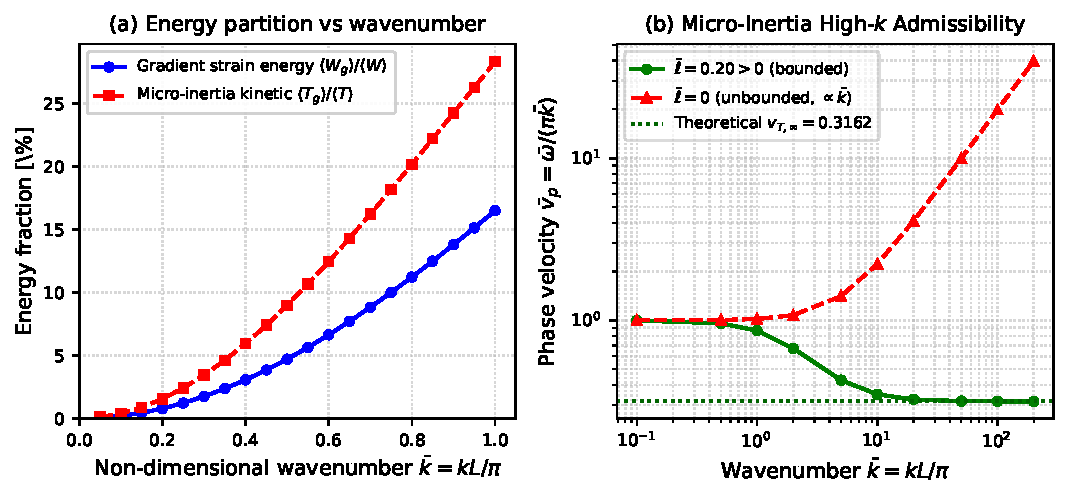
\includegraphics[width=\textwidth]{figures/fig13_energy_microinertia.pdf}
\caption{(a) Gradient-energy fraction $W_g/W$ versus wavenumber. (b) Transverse-branch phase velocity with and without gradient micro-inertia; the finite high-wavenumber limit is specific to the shear branch analyzed here}
\label{fig:energy_microinertia}
\end{figure*}

The transverse shear branch analyzed in Appendix~\ref{app:asymptotics} has the asymptotic limit
\begin{equation}
\begin{split}
\bar{v}_{T,\infty} &= \frac{\bar{l}_{\mathrm{eff}}}{\sqrt{10}\,\bar{\ell}_{\mathrm{i}}} \\
&= \frac{0.20}{\sqrt{10}\times0.20} = \frac{1}{\sqrt{10}} \approx 0.3162.
\end{split}
\label{eq:v_horizon_sec7}
\end{equation}
At $\bar{k}=200$, the computed phase speed with micro-inertia is $0.3163$, within $0.03\%$ of this asymptote. Without micro-inertia, the analytical branch relation grows without bound, and the computed phase speed reaches $39.75$ at $\bar{k}=200$. In Eq.~\eqref{eq:appA_vp}, the gradient-stiffness and micro-inertia corrections to $v_p^2$ both grow as $k^2$; their ratio sets the finite high-wavenumber limit, while setting $\ell_{\mathrm{i}}=0$ removes the inertial denominator term and restores the unbounded trend. This result applies only to the transverse branch and constitutive model studied; it does not establish a speed bound for other branches or models.

\section{Discussion and limitations}
\label{sec:discussion}

In homogeneous Case~H, the rotated characteristic-length tensor changes the gradient-stiffness contribution according to the wave-vector direction relative to its principal axes. The resulting branch shifts are unequal: rotating the tensor can separate neighboring bands along $\Gamma$--$X$ while modes at other wave vectors remain in the same frequency interval. Under the volume-equivalent scaling, changing the aspect ratio lengthens one principal characteristic length while shortening the other, so the two bounding band edges need not move together. Their frequency difference can therefore vary non-monotonically. A positive $\Delta_{GX}$ is therefore a reduced-zone separation along $\Gamma$--$X$ only, with modes elsewhere in the Brillouin zone consistent with the negative complete-gap measure $\Delta_{\mathrm{complete}}\le -0.3235$; without material contrast it is direction-selective spectral separation, not full-zone attenuation of an incident wave. The 42-point map compares evaluated configurations rather than identifying a continuous optimum.

The group-velocity response follows from the same direction-dependent dispersion. Because $\bmv_g=\nabla_{\bmk}\omega$ is normal to a local constant-frequency contour, changes in contour slope alter the angle between the energy-flow direction and the wave vector. Rotating the length tensor reorients these local contour normals and shifts the steering lobes. On the sampled acoustic branch at $\bar{k}=0.5$, the peak deviation is nearly unchanged while its principal direction moves. Orientation therefore redirects the energy flow without materially increasing its peak angular deviation, within the branch, ring, and orientations sampled here.

Case~C adds periodic contrast in both shear modulus and density. The resulting Bloch bands separate Bands~3 and~4 over the sampled Brillouin zone, unlike the path-specific branch separation in homogeneous Case~H. This difference is consistent with the positive complete-gap measure in Case~C and the absence of a complete gap in Case~H. The Case-C gap decreases from $2.5732$ on the $4\times4$ mesh to $1.9179$ on the $64\times64$ mesh and remains unconverged. Because the cases use different material and discretization settings, the comparison is interpretive rather than a controlled parameter sweep; the coarse-mesh Case-C width is not a continuum estimate.

The homogeneous mesh study gives an empirical rate $p=4.17$ over the $4^2$, $8^2$, and $16^2$ levels. The $32^2$ result is resolution-limited and excluded from the fit, so this rate is not a theoretical-order claim. All eight tabulated numerical consistency checks meet their stated criteria; the energy-flux/group-velocity identity, evaluated on closed-form Case-H harmonic fields, holds to $6.91\times10^{-10}$.

The classical AlN/BaTiO$_3$ calculation reproduces the Rytov transfer-matrix relation to $2.22\times10^{-16}$, although the comparison with the published B1 curves stays visual because tabulated source values are unavailable. The two gradient-elastic bilayer cases are reproductions rather than quantitative external validations, since their source parameter conventions are unresolved; no external-validation claim is made for those benchmarks.

For the transverse branch in ~\ref{app:asymptotics}, gradient stiffness raises the phase speed at high wavenumber when micro-inertia is absent. With micro-inertia, the $k^2$ contribution in the numerator of $v_p^2$ is balanced asymptotically by the $k^2$ inertial term in its denominator, leaving a finite limit set by the ratio of the gradient-stiffness and micro-inertia lengths. This is a mechanism-specific result for the branch and constitutive model studied, not a universal bound. More broadly, the model is linear, local, isothermal, and two-dimensional under plane-strain assumptions; it excludes nonlinear gradient effects, dissipation, piezoelectric coupling, and three-dimensional polarization modes.

\section{Conclusions}
\label{sec:conclusions}
\sloppy

This work analyzed orientation-dependent Bloch dispersion in two-dimensional strain-gradient elasticity by combining a rotated ellipsoidal characteristic-length tensor with local Mindlin Form-II gradient elasticity and independent gradient micro-inertia, discretized with a conforming 32-degree-of-freedom BFS element that applies the Bloch phase to both displacement and derivative degrees of freedom.

The main findings are as follows:
\begin{itemize}
  \item In homogeneous Case~H, aspect ratio and orientation shift the zone-edge branches and can open a directional spectral separation along selected directions, but the complete-gap measure remains negative: with no material contrast the effect is a reduced-zone one, and orientation-based tuning provides spectral separation rather than complete attenuation.

  \item At fixed area, varying aspect ratio redistributes the principal length scales, and the sampled directional gap responds non-monotonically. The largest sampled $\Delta_{GX}=0.0677$ occurs at $\theta=0^\circ$, $\mathrm{AR}=7$; this identifies a design point in the evaluated set, not a continuous optimum.

  \item On the acoustic branch, rotating the tensor moves the steering lobes while the peak deviation remains nearly unchanged over the sampled orientations. For the evaluated ring and aspect ratios, orientation selects the energy-flow direction rather than increasing the sampled peak steering magnitude.

  \item Periodic epoxy--YBCO contrast in Case~C yields a positive complete gap between Bands~3 and~4 on every computed finite-element mesh, but its width narrows under refinement. The reported coarse-mesh width is therefore resolution-specific and is not a converged continuum estimate.

  \item For the transverse branch studied, gradient micro-inertia gives a finite high-wavenumber phase-speed limit of $0.3162$. This result is specific to the branch and constitutive model; it is not a bound established for other branches or formulations.

  \item All eight tabulated consistency checks are satisfied, including the energy-flux/group-velocity identity. The heterogeneous-literature comparisons remain qualitative, so the evidence supports the reported within-model trends rather than external agreement for the two-dimensional bands.
\end{itemize}

The formulation is directly applicable to analyzing orientation- and aspect-ratio-dependent directional dispersion and group-velocity steering in homogeneous strain-gradient media, and to complete-gap design in physically periodic, material-contrast media of the kind studied in Case~C. Extending the complete-gap result in Case~C to a mesh-converged estimate is the most direct next step; three-dimensional generalization of the characteristic-length tensor and element would require a corresponding $C^1$ volumetric discretization.


\backmatter

\bmhead{Supplementary information}
The accompanying Supplementary Material provides the complete parameter summary, extended transfer-matrix comparisons and their validation limits, expanded numerical consistency and mesh-convergence diagnostics, and additional Case-C gap-resolution data.

\bmhead{Acknowledgements}
Vipin Gupta acknowledges the Haryana State Higher Education Council (HSHEC), Government of Haryana, for support through the Haryana State Research Fund (HSRF) scheme (Sanction Letter No.~14/66-2026 SPD/HSHEC/HSRF-38).

\section*{Declarations}

\begin{itemize}
\item \textbf{Funding:} This work was supported by the Haryana State Higher Education Council (HSHEC), Government of Haryana, through the Haryana State Research Fund (HSRF) scheme (Sanction Letter No.~14/66-2026 SPD/HSHEC/HSRF-38).
\item \textbf{Competing interests:} The author declares no competing financial or non-financial interests.
\item \textbf{Ethics approval and consent to participate:} Not applicable. Ethics approval was not required because this theoretical and computational study involved no human participants or animals.
\item \textbf{Data availability:} All data that support the findings of this study are included within the article and its accompanying Supplementary Material.
\item \textbf{Code availability:} The custom $C^1$ Bogner--Fox--Schmit finite-element and Bloch--Floquet dispersion routines used in this study are available from the corresponding author upon reasonable request.
\item \textbf{Author contributions:} Vipin Gupta: Conceptualization, Methodology, Software, Validation, Formal analysis, Investigation, Data curation, Writing~--~original draft, Writing~--~review and editing, Visualization, and Funding acquisition.
\end{itemize}

\begin{appendices}
\section{High-Wavenumber Phase Velocity Asymptotics}
\label{app:asymptotics}

We derive the high-wavenumber phase-speed limit for the one-dimensional transverse-shear branch of the strain-gradient model. Without micro-inertia ($\ell_{\mathrm{i}}=0$), the phase velocity grows without bound as $k\to\infty$. With micro-inertia ($\ell_{\mathrm{i}}>0$), it approaches a finite asymptote.

We consider one-dimensional transverse-shear propagation in a Mindlin Form-II gradient-elastic continuum governed by the equation of motion:
\begin{equation}
\mu \frac{\partial^2 u}{\partial x^2} - \frac{1}{10} \mu l_{\mathrm{eff}}^2 \frac{\partial^4 u}{\partial x^4} = \rho \frac{\partial^2 u}{\partial t^2} - \rho \ell_{\mathrm{i}}^2 \frac{\partial^4 u}{\partial x^2 \partial t^2},
\label{eq:appA_pde}
\end{equation}
where $\mu$ is the shear modulus, $\rho$ is the mass density, $l_{\mathrm{eff}}^2 = \hat{\bmk}\cdot\mathbf{L}\cdot\hat{\bmk}$ is the effective characteristic gradient-stiffness length scale (with the factor $1/10$ inherited from the second moment of the 3D ellipsoidal domain), and $\ell_{\mathrm{i}}$ is the micro-inertia length parameter. Substituting the time-harmonic plane wave ansatz $u(x, t) = A e^{\iu(k x - \omega t)}$ into Eq.~\eqref{eq:appA_pde} yields:
\begin{equation}
-\mu k^2 - \frac{1}{10} \mu l_{\mathrm{eff}}^2 k^4 = -\rho \omega^2 - \rho \ell_{\mathrm{i}}^2 \omega^2 k^2.
\label{eq:appA_char}
\end{equation}
Solving the equation gives the dispersion relation:
\begin{equation}
\omega^2(k) = \frac{\mu}{\rho} \frac{k^2 \left( 1 + \frac{1}{10} l_{\mathrm{eff}}^2 k^2 \right)}{1 + \ell_{\mathrm{i}}^2 k^2}.
\label{eq:appA_dispersion}
\end{equation}
The phase velocity $v_p(k) \equiv \omega(k)/k$ is therefore:
\begin{equation}
v_p(k) = \sqrt{\frac{\mu}{\rho}} \sqrt{\frac{1 + \frac{1}{10} l_{\mathrm{eff}}^2 k^2}{1 + \ell_{\mathrm{i}}^2 k^2}} = c_T \sqrt{\frac{1 + \frac{1}{10} l_{\mathrm{eff}}^2 k^2}{1 + \ell_{\mathrm{i}}^2 k^2}},
\label{eq:appA_vp}
\end{equation}
where $c_T = \sqrt{\mu/\rho}$ is the classical acoustic shear wave speed.

\paragraph{Case 1: No micro-inertia ($\ell_{\mathrm{i}} = 0$)}
Setting $\ell_{\mathrm{i}} = 0$ in Eq.~\eqref{eq:appA_vp} yields:
\begin{equation}
v_p(k) = c_T \sqrt{1 + \frac{1}{10} l_{\mathrm{eff}}^2 k^2}.
\label{eq:appA_vp_zero}
\end{equation}
In the short-wave limit ($k \to \infty$), the phase velocity behaves asymptotically as:
\begin{equation}
\lim_{k \to \infty} v_p(k) = \lim_{k \to \infty} \frac{c_T l_{\mathrm{eff}}}{\sqrt{10}} k \to \infty.
\label{eq:appA_unbounded}
\end{equation}
Similarly, the group velocity $v_g(k) = \dif\omega/\dif k$ is given by:
\begin{equation}
\begin{split}
v_g(k) &= c_T \frac{1 + \frac{2}{10} l_{\mathrm{eff}}^2 k^2}{\sqrt{1 + \frac{1}{10} l_{\mathrm{eff}}^2 k^2}} \\
&\sim \frac{2 c_T l_{\mathrm{eff}}}{\sqrt{10}} k \to \infty \quad \text{as } k \to \infty.
\end{split}
\label{eq:appA_vg_unbounded}
\end{equation}
Both phase and group velocities therefore grow without bound at high wavenumbers in this one-dimensional transverse-shear model when micro-inertia is omitted.

\paragraph{Case 2: With micro-inertia ($\ell_{\mathrm{i}} > 0$)}
For $\ell_{\mathrm{i}} > 0$, taking the limit of Eq.~\eqref{eq:appA_vp} as $k \to \infty$ gives:
\begin{equation}
\begin{split}
v_{p,\infty} \equiv \lim_{k \to \infty} v_p(k) &= c_T \lim_{k \to \infty} \sqrt{\frac{\frac{1}{10} l_{\mathrm{eff}}^2 k^2 (1 + \frac{10}{l_{\mathrm{eff}}^2 k^2})}{\ell_{\mathrm{i}}^2 k^2 (1 + \frac{1}{\ell_{\mathrm{i}}^2 k^2})}} \\
&= c_T \frac{l_{\mathrm{eff}}}{\sqrt{10}\,\ell_{\mathrm{i}}}.
\end{split}
\label{eq:appA_vp_bounded}
\end{equation}
With velocity scaled by $c_T = 1.0$, the dimensionless limit is:
\begin{equation}
\bar{v}_{T,\infty} = \frac{\bar{l}_{\mathrm{eff}}}{\sqrt{10}\,\bar{\ell}_{\mathrm{i}}}.
\label{eq:appA_v_horizon}
\end{equation}
For the Case H baseline ($l_{\mathrm{eff}} = l_{\mathrm{iso}} = 0.20\,\mathrm{m}$, $\ell_{\mathrm{i}} = 0.20\,\mathrm{m}$ from Table~\ref{tab:case_params}, with $\bar{l}_{\mathrm{eff}} = 0.20$ and $\bar{\ell}_{\mathrm{i}} = 0.20$), the transverse asymptotic limit is:
\begin{equation}
\bar{v}_{T,\infty} = \frac{0.20}{\sqrt{10} \times 0.20} = \frac{1}{\sqrt{10}} \approx 0.3162.
\label{eq:appA_horizon_val}
\end{equation}
As verified numerically in Section~\ref{sec:microinertia}, the finite element phase velocity at $\bar{k} = 200$ attains $\bar{v}_p = 0.3163$, matching the analytical horizon within $0.03\%$. For this transverse branch, micro-inertia gives a finite high-wavenumber phase-speed limit.

\section{Time-Averaged Energy Flux in Form-II Gradient Elasticity}
\label{app:energy_flux}

This appendix derives the conservation of elastodynamic energy and the explicit form of the time-averaged Poynting-type energy flux vector $\bm{S}$ in a Mindlin Form-II gradient-elastic solid with micro-inertia.

The local balance of mechanical energy is expressed by the continuity relation:
\begin{equation}
\frac{\partial}{\partial t}(W + T) + \nabla \cdot \bm{S} = 0,
\label{eq:appB_poynting_theorem}
\end{equation}
where $W$ and $T$ are the strain and kinetic energy densities defined in Eqs.~\eqref{eq:strain_energy_W} and \eqref{eq:kinetic_energy_T}. Differentiating $W$ and $T$ with respect to time gives:
\begin{align}
\frac{\partial W}{\partial t} &= \sigma_{ij} \dot{\varepsilon}_{ij} + \tau_{ijk} \dot{\eta}_{ijk} = \sigma_{ij} \dot{u}_{i,j} + \tau_{ijk} \dot{u}_{i,jk}, \label{eq:appB_dWdt} \\
\frac{\partial T}{\partial t} &= \rho \dot{u}_i \ddot{u}_i + \rho \ell_{\mathrm{i}}^2 \dot{u}_{i,j} \ddot{u}_{i,j}. \label{eq:appB_dTdt}
\end{align}
Expanding the spatial derivative terms in Eq.~\eqref{eq:appB_dWdt} using the product rule:
\begin{align}
\sigma_{ij} \dot{u}_{i,j} &= (\sigma_{ij} \dot{u}_i)_{,j} - \sigma_{ij,j} \dot{u}_i, \label{eq:appB_id1} \\
\tau_{ijk} \dot{u}_{i,jk} &= (\tau_{ijk} \dot{u}_{i,j})_{,k} - \tau_{ijk,k} \dot{u}_{i,j} \notag \\
&= (\tau_{ikj} \dot{u}_{i,k})_{,j} - (\tau_{ijk,k} \dot{u}_i)_{,j} + \tau_{ijk,kj} \dot{u}_i. \label{eq:appB_id2}
\end{align}
Similarly, the micro-inertial rate term in Eq.~\eqref{eq:appB_dTdt} expands to:
\begin{equation}
\rho \ell_{\mathrm{i}}^2 \dot{u}_{i,j} \ddot{u}_{i,j} = (\rho \ell_{\mathrm{i}}^2 \dot{u}_i \ddot{u}_{i,j})_{,j} - \rho \ell_{\mathrm{i}}^2 \dot{u}_i \ddot{u}_{i,jj}.
\label{eq:appB_id3}
\end{equation}
Adding Eqs.~\eqref{eq:appB_dWdt} and \eqref{eq:appB_dTdt} and substituting the equation of motion $\sigma_{ij,j} - \tau_{ijk,jk} = \rho(\ddot{u}_i - \ell_{\mathrm{i}}^2 \ddot{u}_{i,jj})$ from Eq.~\eqref{eq:strong_form} cancels the bulk terms:
\begin{equation}
\frac{\partial (W + T)}{\partial t} = \left[ (\sigma_{ij} - \tau_{ijk,k}) \dot{u}_i + \tau_{ikj} \dot{u}_{i,k} + \rho \ell_{\mathrm{i}}^2 \dot{u}_i \ddot{u}_{i,j} \right]_{,j}.
\label{eq:appB_energy_step}
\end{equation}
Comparing Eq.~\eqref{eq:appB_energy_step} with Eq.~\eqref{eq:appB_poynting_theorem} gives the instantaneous energy flux vector $S_j$:
\begin{equation}
S_j = -(\sigma_{ij} - \tau_{ijk,k}) \dot{u}_i - \tau_{ikj} \dot{u}_{i,k} - \rho \ell_{\mathrm{i}}^2 \dot{u}_i \ddot{u}_{i,j}.
\label{eq:appB_S_instant}
\end{equation}
The terms in Eq.~\eqref{eq:appB_S_instant} describe classical traction power modified by the double-stress divergence, double-stress power acting on velocity gradients, and a micro-inertial term.

For time-harmonic fields represented in complex notation $\bmu(\bmx, t) = \mathrm{Re}[\tilde{\bmu}(\bmx) e^{-\iu \omega t}]$, the cycle-averaged energy flux $\langle S_j \rangle = \frac{1}{\mathcal{T}}\int_0^{\mathcal{T}} S_j\,\dif t$ is given by:
\begin{equation}
\begin{split}
\langle S_j \rangle = -\frac{1}{2} \mathrm{Re} \Big[ &(\tilde{\sigma}_{ij} - \tilde{\tau}_{ijk,k}) (-\iu \omega \tilde{u}_i)^* + \tilde{\tau}_{ikj} (-\iu \omega \tilde{u}_{i,k})^* \\
&+ \rho \ell_{\mathrm{i}}^2 (-\iu \omega \tilde{u}_i) (-\omega^2 \tilde{u}_{i,j})^* \Big].
\end{split}
\label{eq:appB_S_cycle}
\end{equation}
Integrating over the unit cell $\Omega_{\mathrm{cell}}$, the cycle-averaged energy flux $\langle \bm{S} \rangle$ and stored energy satisfy:
\begin{equation}
\bm{v}_g = \frac{\langle \bm{S} \rangle}{\langle W \rangle + \langle T \rangle},
\label{eq:appB_vg_identity}
\end{equation}
This identity relates the group velocity $\bm{v}_g = \nabla_{\bmk}\omega$ to the cell-averaged energy flux and stored energy. Table~\ref{tab:consistency_suite} lists a group-velocity/energy-flux residual of $6.91\times10^{-10}$. It is obtained from closed-form Case-H harmonic fields evaluated with the sign convention of Eq.~\eqref{eq:appB_S_cycle}, comparing the cycle-averaged flux $\langle\bm{S}\rangle/(\langle W\rangle+\langle T\rangle)$ against a central-difference estimate of $\nabla_{\bmk}\omega$ for both acoustic branches and multiple in-plane directions.

\end{appendices}

\bibliography{references_final_v7}

\end{document}
